
%% bare_conf.tex
%% V1.4b
%% 2015/08/26
%% by Michael Shell
%% See:
%% http://www.michaelshell.org/
%% for current contact information.
%%
%% This is a skeleton file demonstrating the use of IEEEtran.cls
%% (requires IEEEtran.cls version 1.8b or later) with an IEEE
%% conference paper.
%%
%% Support sites:
%% http://www.michaelshell.org/tex/ieeetran/
%% http://www.ctan.org/pkg/ieeetran
%% and
%% http://www.ieee.org/

%%*************************************************************************
%% Legal Notice:
%% This code is offered as-is without any warranty either expressed or
%% implied; without even the implied warranty of MERCHANTABILITY or
%% FITNESS FOR A PARTICULAR PURPOSE!
%% User assumes all risk.
%% In no event shall the IEEE or any contributor to this code be liable for
%% any damages or losses, including, but not limited to, incidental,
%% consequential, or any other damages, resulting from the use or misuse
%% of any information contained here.
%%
%% All comments are the opinions of their respective authors and are not
%% necessarily endorsed by the IEEE.
%%
%% This work is distributed under the LaTeX Project Public License (LPPL)
%% ( http://www.latex-project.org/ ) version 1.3, and may be freely used,
%% distributed and modified. A copy of the LPPL, version 1.3, is included
%% in the base LaTeX documentation of all distributions of LaTeX released
%% 2003/12/01 or later.
%% Retain all contribution notic
%%es and credits.
%% ** Modified files should be clearly indicated as such, including  **
%% ** renaming them and changing author support contact information. **
%%************************************************uppfylla*************************


% *** Authors should verify (and, if needed, correct) their LaTeX system  ***
% *** with the testflow diagnostic prior to trusting their LaTeX platform ***
% *** with production work. The IEEE's font choices and paper sizes can   ***
% *** trigger bugs that do not appear when using other class files.       ***                          ***
% The testflow support page is at:
% http://www.michaelshell.org/tex/testflow/



\documentclass[conference,a4paper]{IEEEtran}
% Some Computer Society conferences also require the compsoc mode option,
% but others use the standard conference format.
%
% If IEEEtran.cls has not been installed into the LaTeX system files,
% manually specify the path to it like:
\usepackage{color, colortbl}
\usepackage[table]{xcolor}
\usepackage{tabu}
\usepackage[utf8]{inputenc}
\usepackage[swedish]{babel}
\usepackage[pdftex]{graphicx}
\usepackage{hyperref}
\usepackage{pdfpages}
\usepackage{float}
\usepackage{pax}
\usepackage{array}
\usepackage{dblfloatfix}


% Från https://tex.stackexchange.com/a/126542
\newcommand\Tstrut{\rule{0pt}{2.6ex}}       % "top" strut
\newcommand\Bstrut{\rule[-0.9ex]{0pt}{0pt}} % "bottom" strut
\newcommand{\TBstrut}{\Tstrut\Bstrut} % top&bottom struts

\graphicspath{{Images/}}
\DeclareGraphicsExtensions{.pdf,.png,.jpg}
% correct bad hyphenation here
\hyphenation{op-tical net-works semi-conduc-tor}

\begin{document}
%
% paper title
% Titles are generally capitalized except for words such as a, an, and, as,
% at, but, by, for, in, nor, of, on, or, the, to and up, which are usually
% not capitalized unless they are the first or last word of the title.
% Linebreaks \\ can be used within to get better formatting as desired.
% Do not put math or special symbols in the title.
\title{Vad är en bra projektmetod för små IT-projekt?}


% author names and affiliations
% use a multiple column layout for up to three different
% affiliations
\author
    {
      \IEEEauthorblockN{Sebastian Heimlén\textsuperscript{1},
        Henrik Björklund\textsuperscript{2},
        Yobart Amino\textsuperscript{3},
        Teo Klestrup Röijezon\textsuperscript{4}}
        \IEEEauthorblockA{\textit{KTH Royal Institute of Technology}
          \textit{Isafjordsgatan 22, 164 40 Kista, Sweden}\\
          \texttt{\textsuperscript{1}heimlen@kth.se}\\
          \texttt{\textsuperscript{2}hebjo@kth.se}\\
          \texttt{\textsuperscript{3}yobart@kth.se}\\
          \texttt{\textsuperscript{4}teo@nullable.se, roijezon@kth.se}
         }
    }

% make the title area
\maketitle

% As a general rule, do not put math, special symbols or citations
% in the abstract
\begin{abstract}
  this is an abstract.

  \textbf{\textit{keywords} - with keywords}
\end{abstract}

\IEEEpeerreviewmaketitle

\section{Om detta dokument och undersökning}
Detta dokument är ett försök att på ett vetenskapligt sätt undersöka projektmetoder inom små IT-projekt. Dokumentet är också delvis en träning på att skriva vetenskapliga rapporter och en övning inför examensarbetet. Dokumentet riktar sig mot akademin och specifikt mot kursens examinator som kommer att utvärdera rapporten enligt ''Blooms taxonomi'' \cite{krathwohl10}.

Rapportens disposition är som följer. Sektion \ref{sec:intro} introducerar rapporten. Sektion \ref{sec:teori} redovisar bakomliggande teori och ingenjörspraxis. Sektion \ref{sec:under} redovisar vår undersökningsmetod. Sektion \ref{sec:genom} beskriver genomförandet. Sektion \ref{sec:res} redovisar resultatet av undersökningen. I sektion \ref{sec:analys} analyseras undersökningen och eventuella förbättringsförslag lämnas. I sektion \ref{sec:disk} diskuteras undersökningen och resultatet av undersökningen. Sektion \ref{sec:slutord} innehåller slutord.

Detta dokuments trovärdighet anses vara hög, då undersökningsmetoden som använts är förankrad i Anderssons och Ekholms rapport som avhandlar vetenskaplighet i IT-projekt \cite{Andersson02}, vilket i sin tur leder till att resultaten är framtagna på ett vetenskapligt sätt. De projektmetoder vi undersöker är erkända och välanvanda inom IT-projekt, och dokumentet refererar till erkända böcker, tidsskrifter samt vetenskapliga texter. Dessa egenskaper bygger tillsammans upp projektets trovärdighet och vi är övertygade om att en likadan undersökning med lika många deltagare och samma förutsättningar skulle komma fram till så gott som samma slutsatser som vi har gjort.

\section{Introduktion} \label{sec:intro}

\subsection{Bakgrund}
Detta dokument är en del av examinationen i kursen ''Projekt och projektmetoder'' i vilket studenter i små grupper genomför ett IT-projekt som innefattar både hårdvara, mjukvara, datornätverk samt elektronik. Syftet med att genomföra projektet är att undersöka samt analysera olika projektmetoder, dessa analyser ska sedan diskuteras och framföras i denna rapport för att kunna besvara frågeställningen ''Vad är en bra projektmetod för små IT-projekt''.

Kursens syfte är att fördjupa studenternas kunskap inom projektmetodik och skall fungera som en förberedelse inför både examensarbete samt det fortsatta arbetslivet efter examen. Kursens projektgrupper består av både data- samt elektrostudenter, och tanken bakom detta är att studenter från de olika programmen har olika expertisområden, vilket leder till att olika studenter har olika ansvarsområden inom projektgruppen, ett mål med kursen är att projektgruppen tillsammans ska utvecklas och dela med sig av sin kunskap, vilket leder till att samtliga medlemmar ytterliggare utvecklas på en personlig nivå.

\subsection{Problemformulering}
Den övergripande frågeställningen är som tidigare nämnt ''Vad är en bra projektmetod för små IT-projekt?''. För att besvara denna frågeställning måste gruppen först undersöka samt komma överens om vad en bra projektmetod är. En vettig utgångspunkt för att beskriva detta är Eklunds åtagandetriangel \cite[s. 128-129]{Eklund14}.

En bra projektmetod kan då beskrivas som en metod där projektgruppen på ett strukturerat och planerat vis tar fram en produkt som tillfredställer kundens krav och ej överskrider projektets budget vad gäller tid och kostnad. Den innefattar även hjälpmedel som underlättar och förbättrar arbetsgången och tillåter projektgruppen att snabbt och ofta ändra arbetssätt, arbetsbörda och/eller förväntat resultatet av projektarbetet, då skiftande krav och oförutsedda problem är en vanlig företeelse i IT-projekt som måste hanteras när de dyker upp.

Efter att ha sanktionerat denna definition av vad en bra projektmetod är blir det betydligt enklare och tydligare att resonera kring den övergripande frågeställningen.
\subsection{Undersökningsstrategi/lösningsstrategi}
Strategin för att undersöka och hitta svar till denna frågeställning har varit att genomföra en fallstudie i vilken projektgruppen genomfört ett litet IT-projekt. Inom detta projekt testas en variant på Scrum-metoden, med mindre inslag från Kanban, och varje medlem har tagit en specifik roll i projektet. Det är sedan varje medlems uppgift att inom denna roll experimentellt under projektets gång samla in information och intryck om vilka projektmetoder som fungerar bra och varför inom den specifika roll medlemmen besitter. Dessa intryck ska sedan analyseras och slutsatser skall dras, och det är dessa analyser och slutsatser som denna rapport avser avhandla.

\subsection{Relaterade arbeten}
Inga relaterade arbeten har hittats.

\subsection{Avgränsningar}
Teorierna i denna rapport avgränsas genom att endast Scrum-metoden tas upp, samt relativa teorier om dessa metoder. Dessa teorier begränsas till stor del av givna artiklar och dokument med viss komplimenterande dokument. Utöver detta så avgränsas också teorierna då projektet genomförs i en studiemiljö i grupper av studenter och samtliga grupper utför samma projektuppdrag.

\section{Teori och ingenjörspraxis} \label{sec:teori}
Detta kapitel listar och i viss mån beskriver teorier och ingenjörspraxis som använts i undersökningen. Det finns två underkapitel, Litteraturstudie och Förstudie.
\subsection{Litteraturstudie}
I genomförandet av denna fallstudie har flera källor konsulterats, och i detta kapitel anges dessa källor. Förutom de källor som anges finns förmodligen andra, och möjligtvis bättre, källor som ej konsulterats.\\

\noindent \textbf{Övergripande källor för hela projektet}
\begin{itemize}
\item Boken \textit{Software Engineering} av Ian Sommerville \cite[kap. 1,2,3]{Sommerville10}.
\\
\item Handboken \textit{Scrum and XP from the Trenches} av Henrik Kniberg \cite{Kniberg07}.
\\
\item Handboken \textit{KanBan och Scrum, få det bästa av två världar} av Henrik Kniberg och Mattias Skarin \cite{Kniberg10}.
\\
\item Artikeln \textit{Industrial Scale Agile, from Craft to Engineering} av Ivar Jacobson, Ian Spence och Ed Seidewitz \cite{Jacobson16}.
\\
\item Webbsidan \textit{Essence Kernel} av Ivar Jacobson \cite{ivarjacobson2017}.
\\
\end{itemize}

\noindent \textbf{Kundrepresentant (Henrik Björklund}
\begin{itemize}
\item \textit{Software Engineering} av Ian Sommerville \cite[kap. 4]{Sommerville10}. Dessa kapitel behandlar kravspecifikationer.
\item \textit{USE-CASE 2.0 The Guide to Succeeding with Use Cases} av Ivar Jacobson, Ian Spence, Kurt Bittner \cite{Jacobson11}. En guide hur kravhantering kan ske.
\\
\end{itemize}

\noindent \textbf{Arkitekt/analytiker (Teo Klestrup Röijezon)}
\begin{itemize}
\item Artikeln \textit{The “4+1” View Model of Software Architecture} av Philippe Kruchten \cite{Kruchten95}.
\item Artikeln \textit{Modeling Web Application Architectures with UML} av Jim Conallen \cite{Conallen99}.
\\
\end{itemize}

\noindent \textbf{Utvecklare}\\
\indent Denna roll existerar i projektet, men det har ej varit en del av undersökningen och vi utelämnar därför rollen ur rapporten.\\
\\
\noindent \textbf{Testare (Yobart Amino)}
\begin{itemize}
\item  \textit{Software Engineering}, Ian Sommerville \cite[kap.1-3,8]{Sommerville10}. De här kapitlen berör teststrategier och testplaner.
\item \textit{Test och kvalitetssäkring av IT-system}, Ulf Eriksson \cite{eriksson_2008}.  Berör olika tekniker, arbetssätt och verktyg för testning.
\\
\\
\end{itemize}

\noindent \textbf{Ledning och styrning (Sebastian Heimlén)}
\begin{itemize}
\item \textit{Software Engineering} av Ian Sommerville \cite[kap. 22,23,26]{Sommerville10}. Dessa kapitel behandlar projektmetodik.
\\
\item Rapporten \textit{Vetenskaplighet - Utvärdering av tre implementeringsprojekt inom IT Bygg och Fastighet 2002} skriven av Niclas Andersson och Anders Ekholm \cite{Andersson02}.
\\
\item Boken \textit{Arbeta i projekt - individen, gruppen, ledaren} av Sven Eklund \cite{Eklund14}.
\\
\end{itemize}

\subsection{Förstudie}
Enligt undersökningsstrategin så skall någon projektmetod prövas i ett praktiskt projekt och utifrån de erfarenheter som fås görs en värdering av använda metoder. Frågan är då vilken ansats av projektmetod som skall användas.

\subsection{Föreslagen ansats}
Eftersom erfarenheten av projektarbete hos studenterna i denna kurs är liten så fanns det ett färdigt förslag till ansats av projektmetod. Tidigare kursomgångar och lärarens förslag har mynnat ut i följande ansats som studenterna själva får välja att använda rakt av eller modifiera till sitt tycke. Projektmetoden framgår med god tydlighet av de arbetstavlor som definierats i ansatsen, se figur \ref{forslagsprintbacklog}, \ref{forslagriktigsprint}, \ref{forslagproductbacklog} och \ref{forslagriktigproduct}.

Den angivna ansatsen innehöll en tavla med två sidor, där ena sidan, den interna, använde sig av en modiferad Kanban metodik, där olika uppgifter kunde följas i vilka stader dom var i, samt hjälpmedel för att se hur projektet fortlöpte (Burndown), även plats för arkitekturen och test fanns på ena sidan. Den andra publika sidan innehöll officiella dokument som förklade vision hos produkten, samt andra hjälp dokument. Även en övergripande User stories enligt \cite{Jacobson11} samt färdiga slices presenterades där för kund och andra intressenter att se. Samt dokument som visade planeringen utav tid och milstoplar i form av ett GANTT-diagram fanns på den publika sidan.

\subsubsection{Anslagstavla}

\begin{figure}[H]
\centering
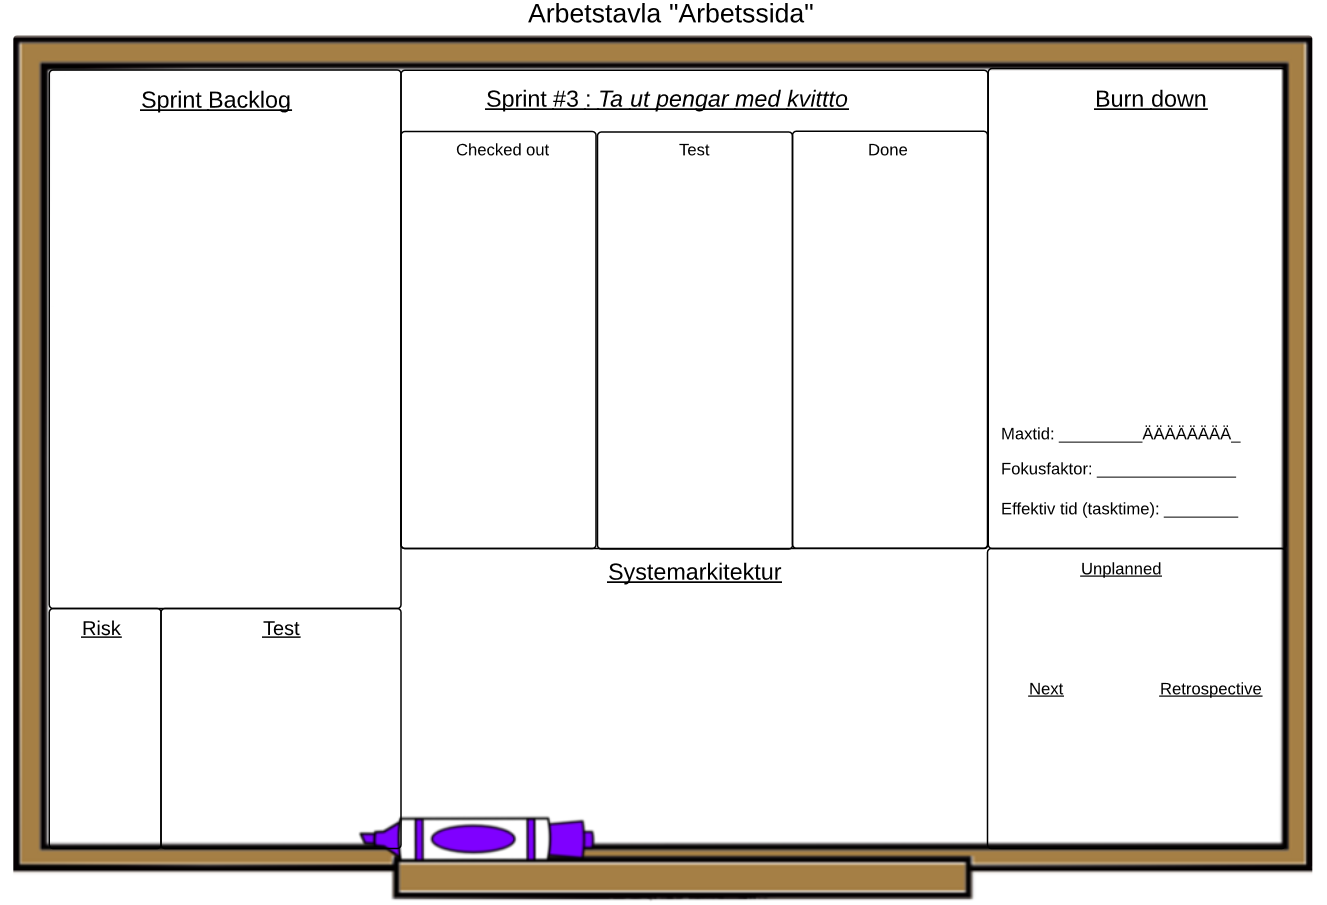
\includegraphics[width=3in]{forslagsprintbacklog}
% where an .eps filename suffix will be assumed under latex,
% and a .pdf suffix will be assumed for pdflatex; or what has been declared
\DeclareGraphicsExtensions.
\caption{Föreslaget Exempel på en intern sida för projektgruppen.}
\label{forslagsprintbacklog}
\end{figure}

\begin{figure}[H]
\centering
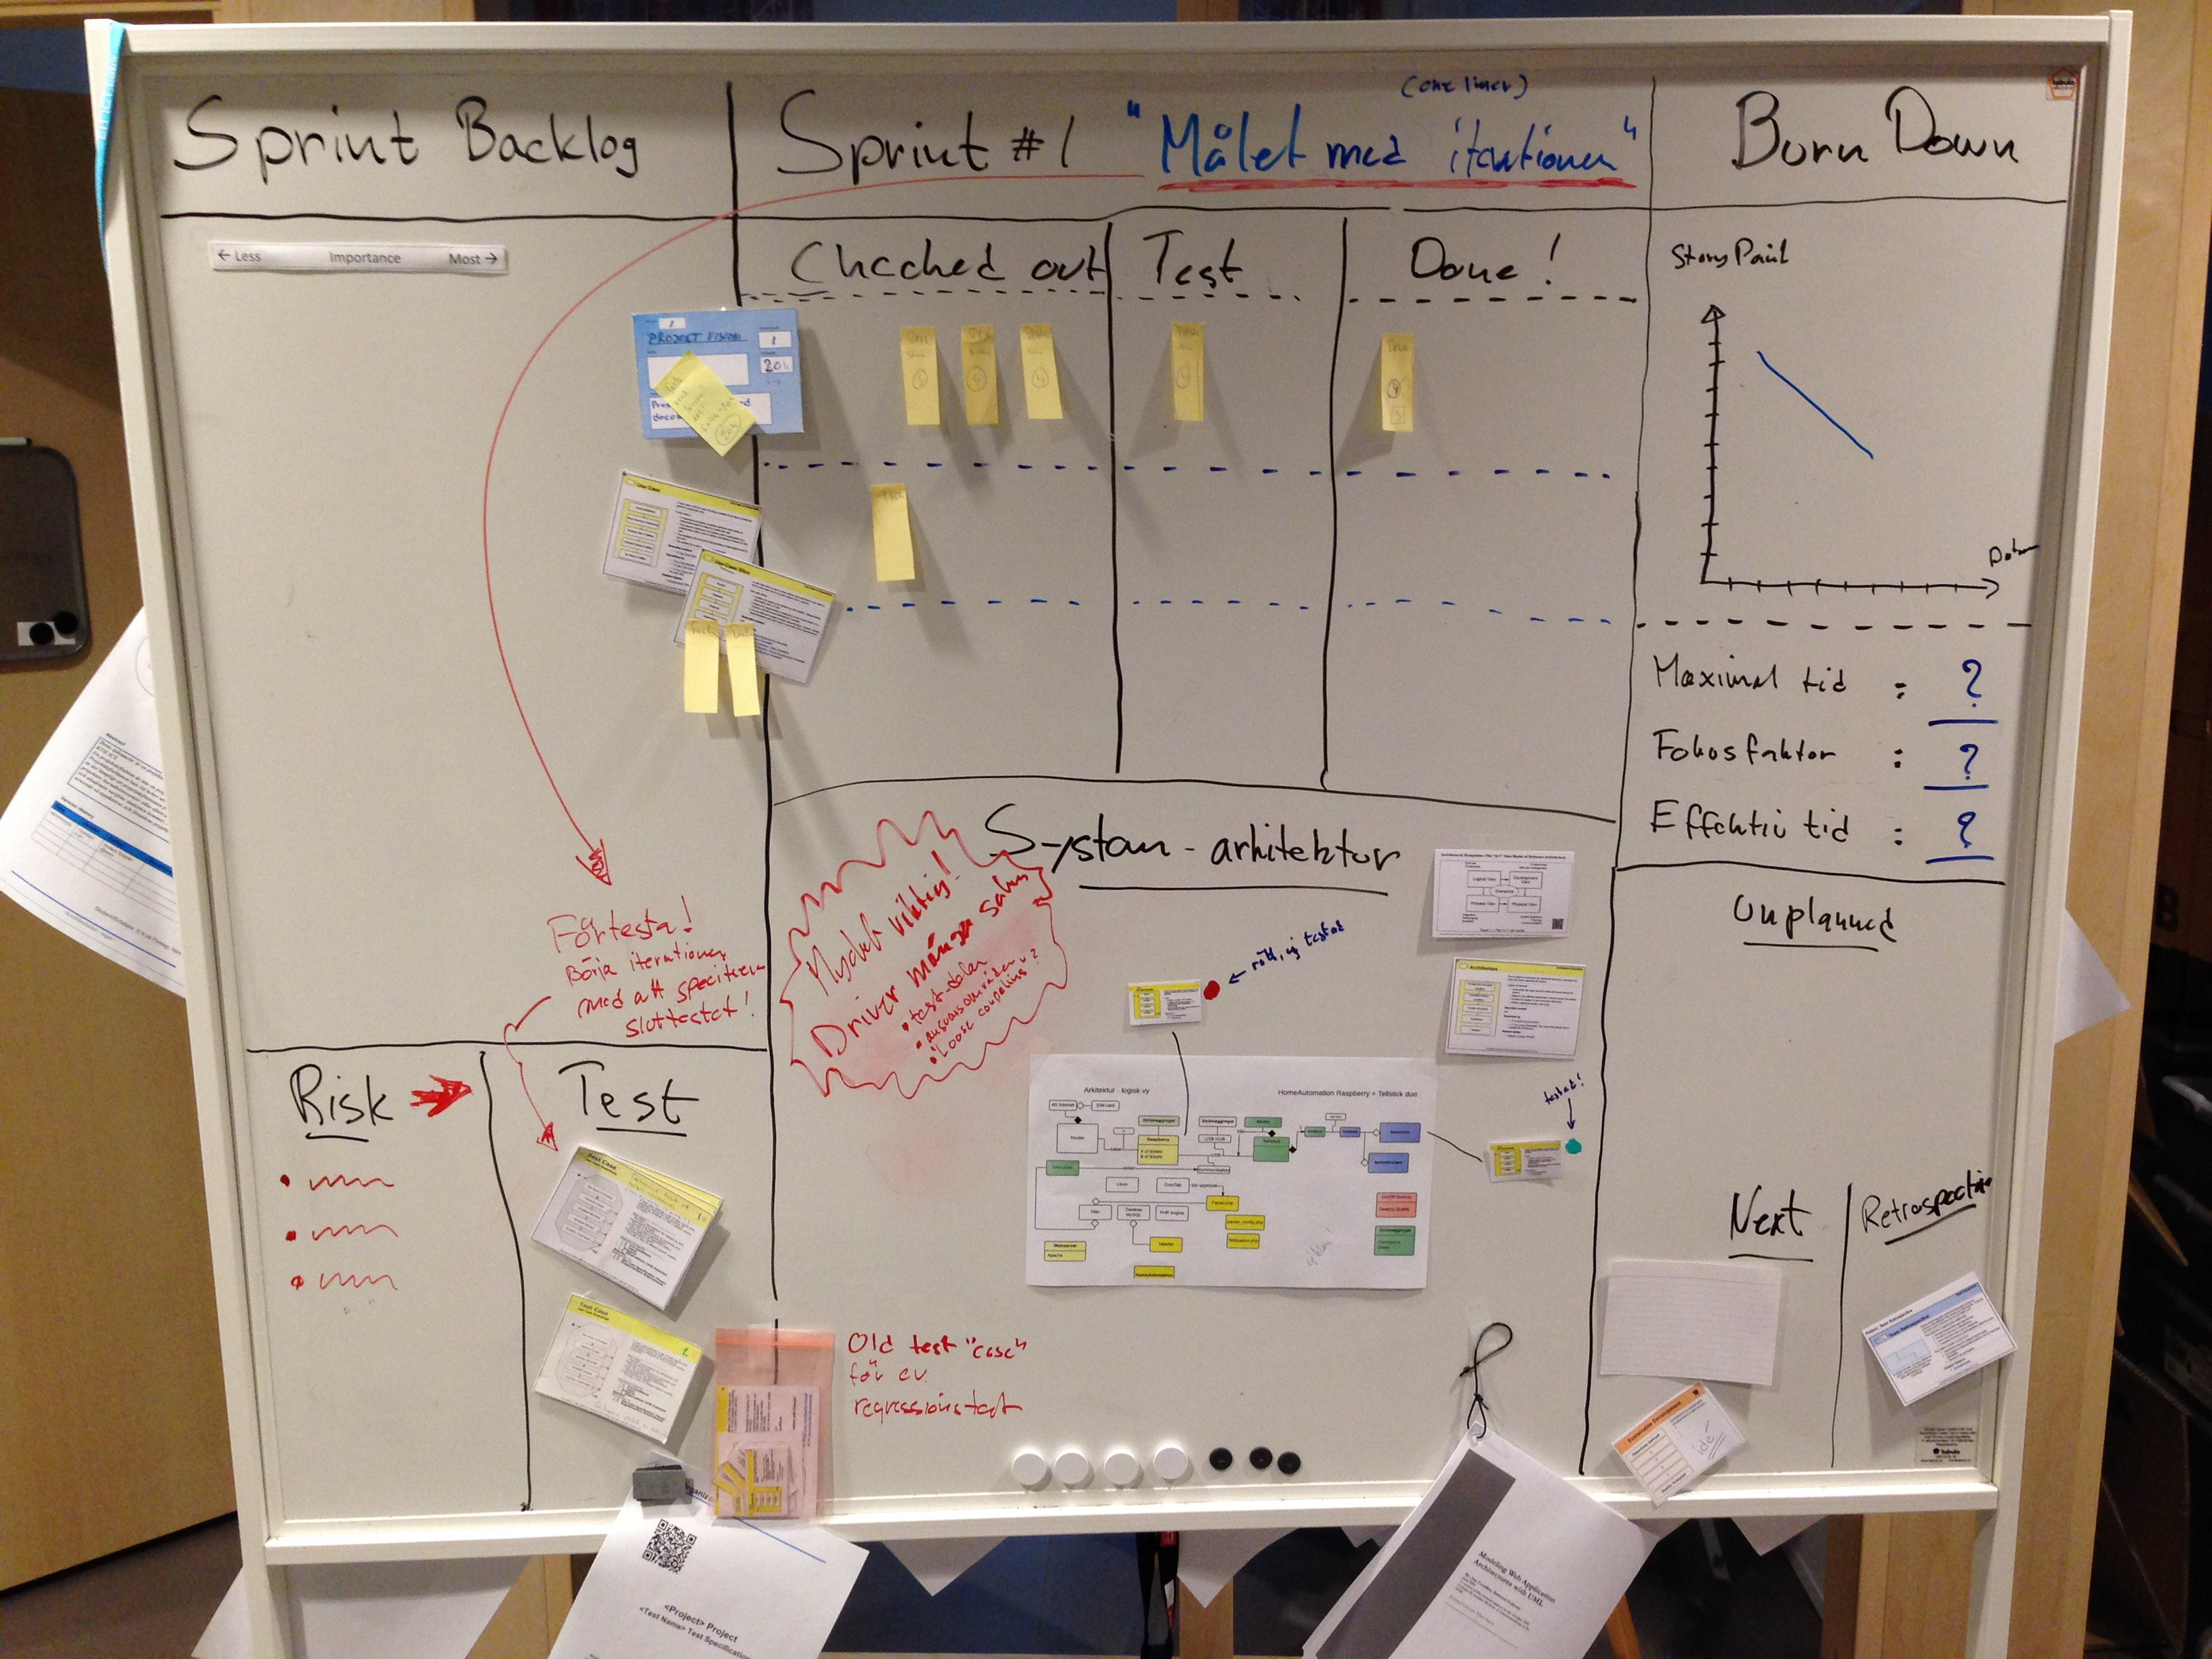
\includegraphics[width=3in]{forslagriktigsprint}
% where an .eps filename suffix will be assumed under latex,
% and a .pdf suffix will be assumed for pdflatex; or what has been declared
\DeclareGraphicsExtensions.
\caption{Demonstration av den föreslagna interna sidan för projektgruppen.}
\label{forslagriktigsprint}
\end{figure}

\begin{figure}[H]
\centering
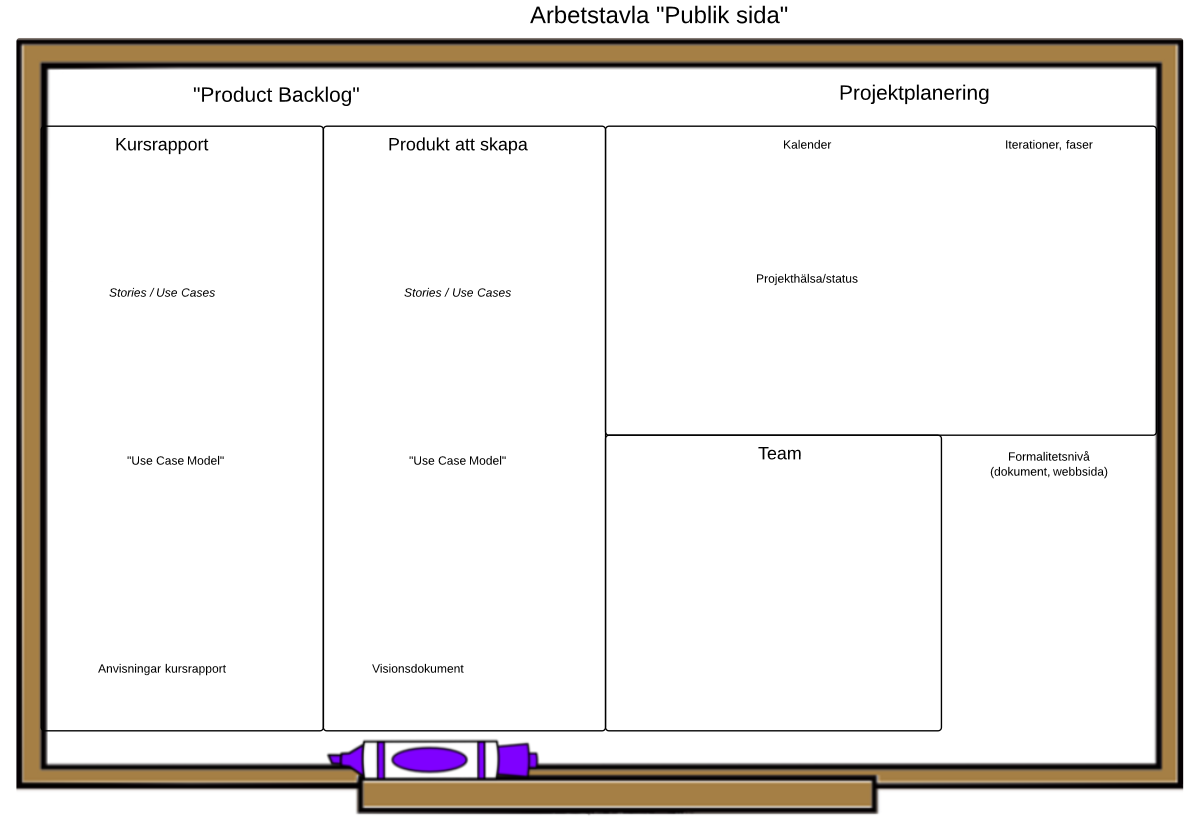
\includegraphics[width=3in]{forslagproductbacklog}
% where an .eps filename suffix will be assumed under latex,
% and a .pdf suffix will be assumed for pdflatex; or what has been declared
\DeclareGraphicsExtensions.
\caption{Föreslaget Exempel på en publik sida för projektgruppen.}
\label{forslagproductbacklog}
\end{figure}

\begin{figure}[H]
\centering
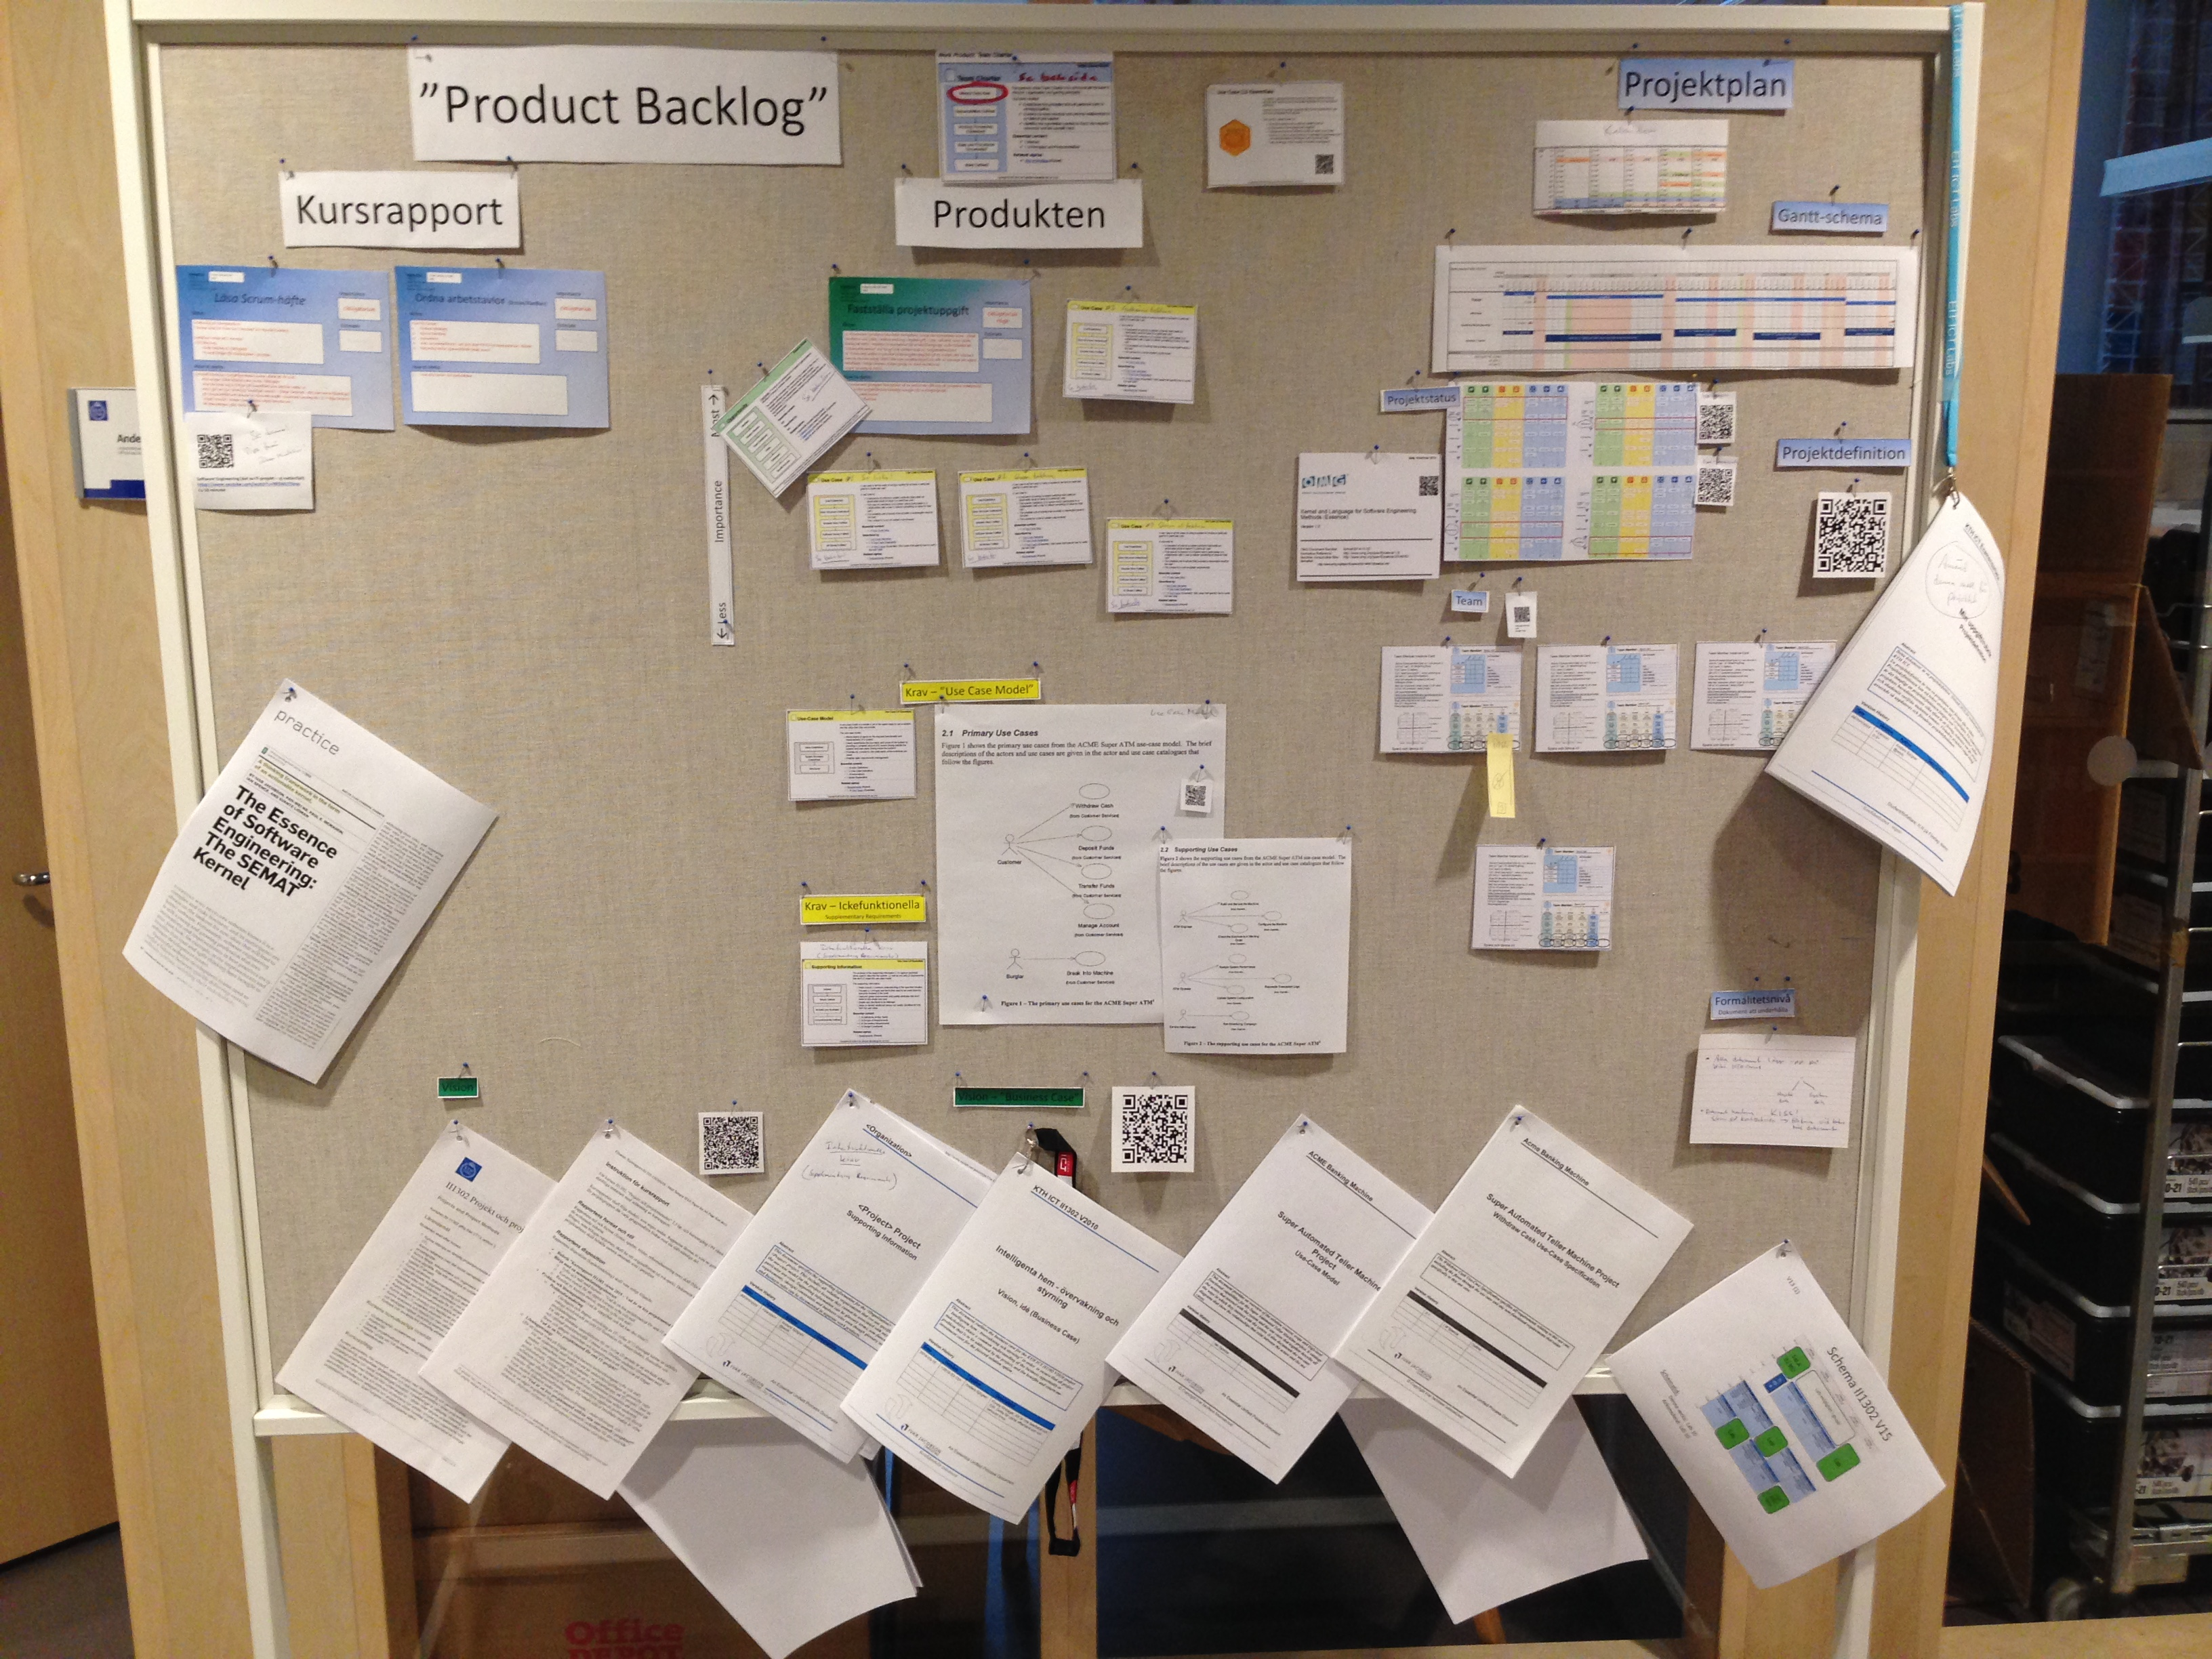
\includegraphics[width=3in]{forslagriktigproduct}
% where an .eps filename suffix will be assumed under latex,
% and a .pdf suffix will be assumed for pdflatex; or what has been declared
\DeclareGraphicsExtensions.
\caption{Demonstration av den föreslagna publika sidan för projektgruppen.}
\label{forslagriktigproduct}
\end{figure}

\begin{figure}[H]
\centering
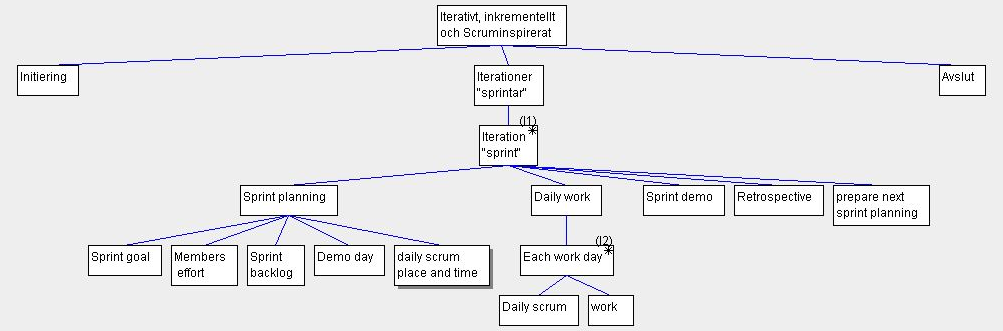
\includegraphics[width=3.5in]{scrum}
% where an .eps filename suffix will be assumed under latex,
% and a .pdf suffix will be assumed for pdflatex; or what has been declared
\DeclareGraphicsExtensions.
\caption{Scruminspirereade projektaktiviteter.}
\label{scruminspo}
\end{figure}

\subsection{Vald ansats}
Då litteraturstudie och kursteori i form av föreläsningar skett löpande under kursen så har projektgruppens egna förstudie gjort likaså. Detta har lett till att den föreslagna ansatsen iterativt förändrats och formats allt eftersom projektgruppens undersökning fortskridit.
Resultatet av förstudien är att metoderna, som anges i följande kapitel, har valts för undersökningens genomförande.
Den slutgiltiga tavlan som då växte fram bestod utav en intern sida där Kanban utformningen från den förslagna ansatsen behölls, dock så migrerades stora delar av User case och tillhörande stories och task till Trello. En utvecklad version av User storyn som publicerades på den publika sidan placerades här, med mera noggran teknisk beskrivning, för att hjälpa utvecklingsteamet att skapa en bättre bild hur produktens alla delar samverkade.

Den publika sidan blev uppdelad i huvudsakligen två delar, där formella dokument om kursrapporten publicerades samt de formella dokument om produkten placerads även här. Viss användning av projektets planering visades på den publika sidan som ett GANTT-diagram, men valda milstoplar, samt ett kort från Ivar Jacobson \cite{Jacobson11} där besökare lätt kunde se hur arbetet hade fortlöpte i hänsyn till ett antal olika faktorer, så som produkten, teamdynamiken samt de komersiella delarna.

\begin{figure}[H]
\centering
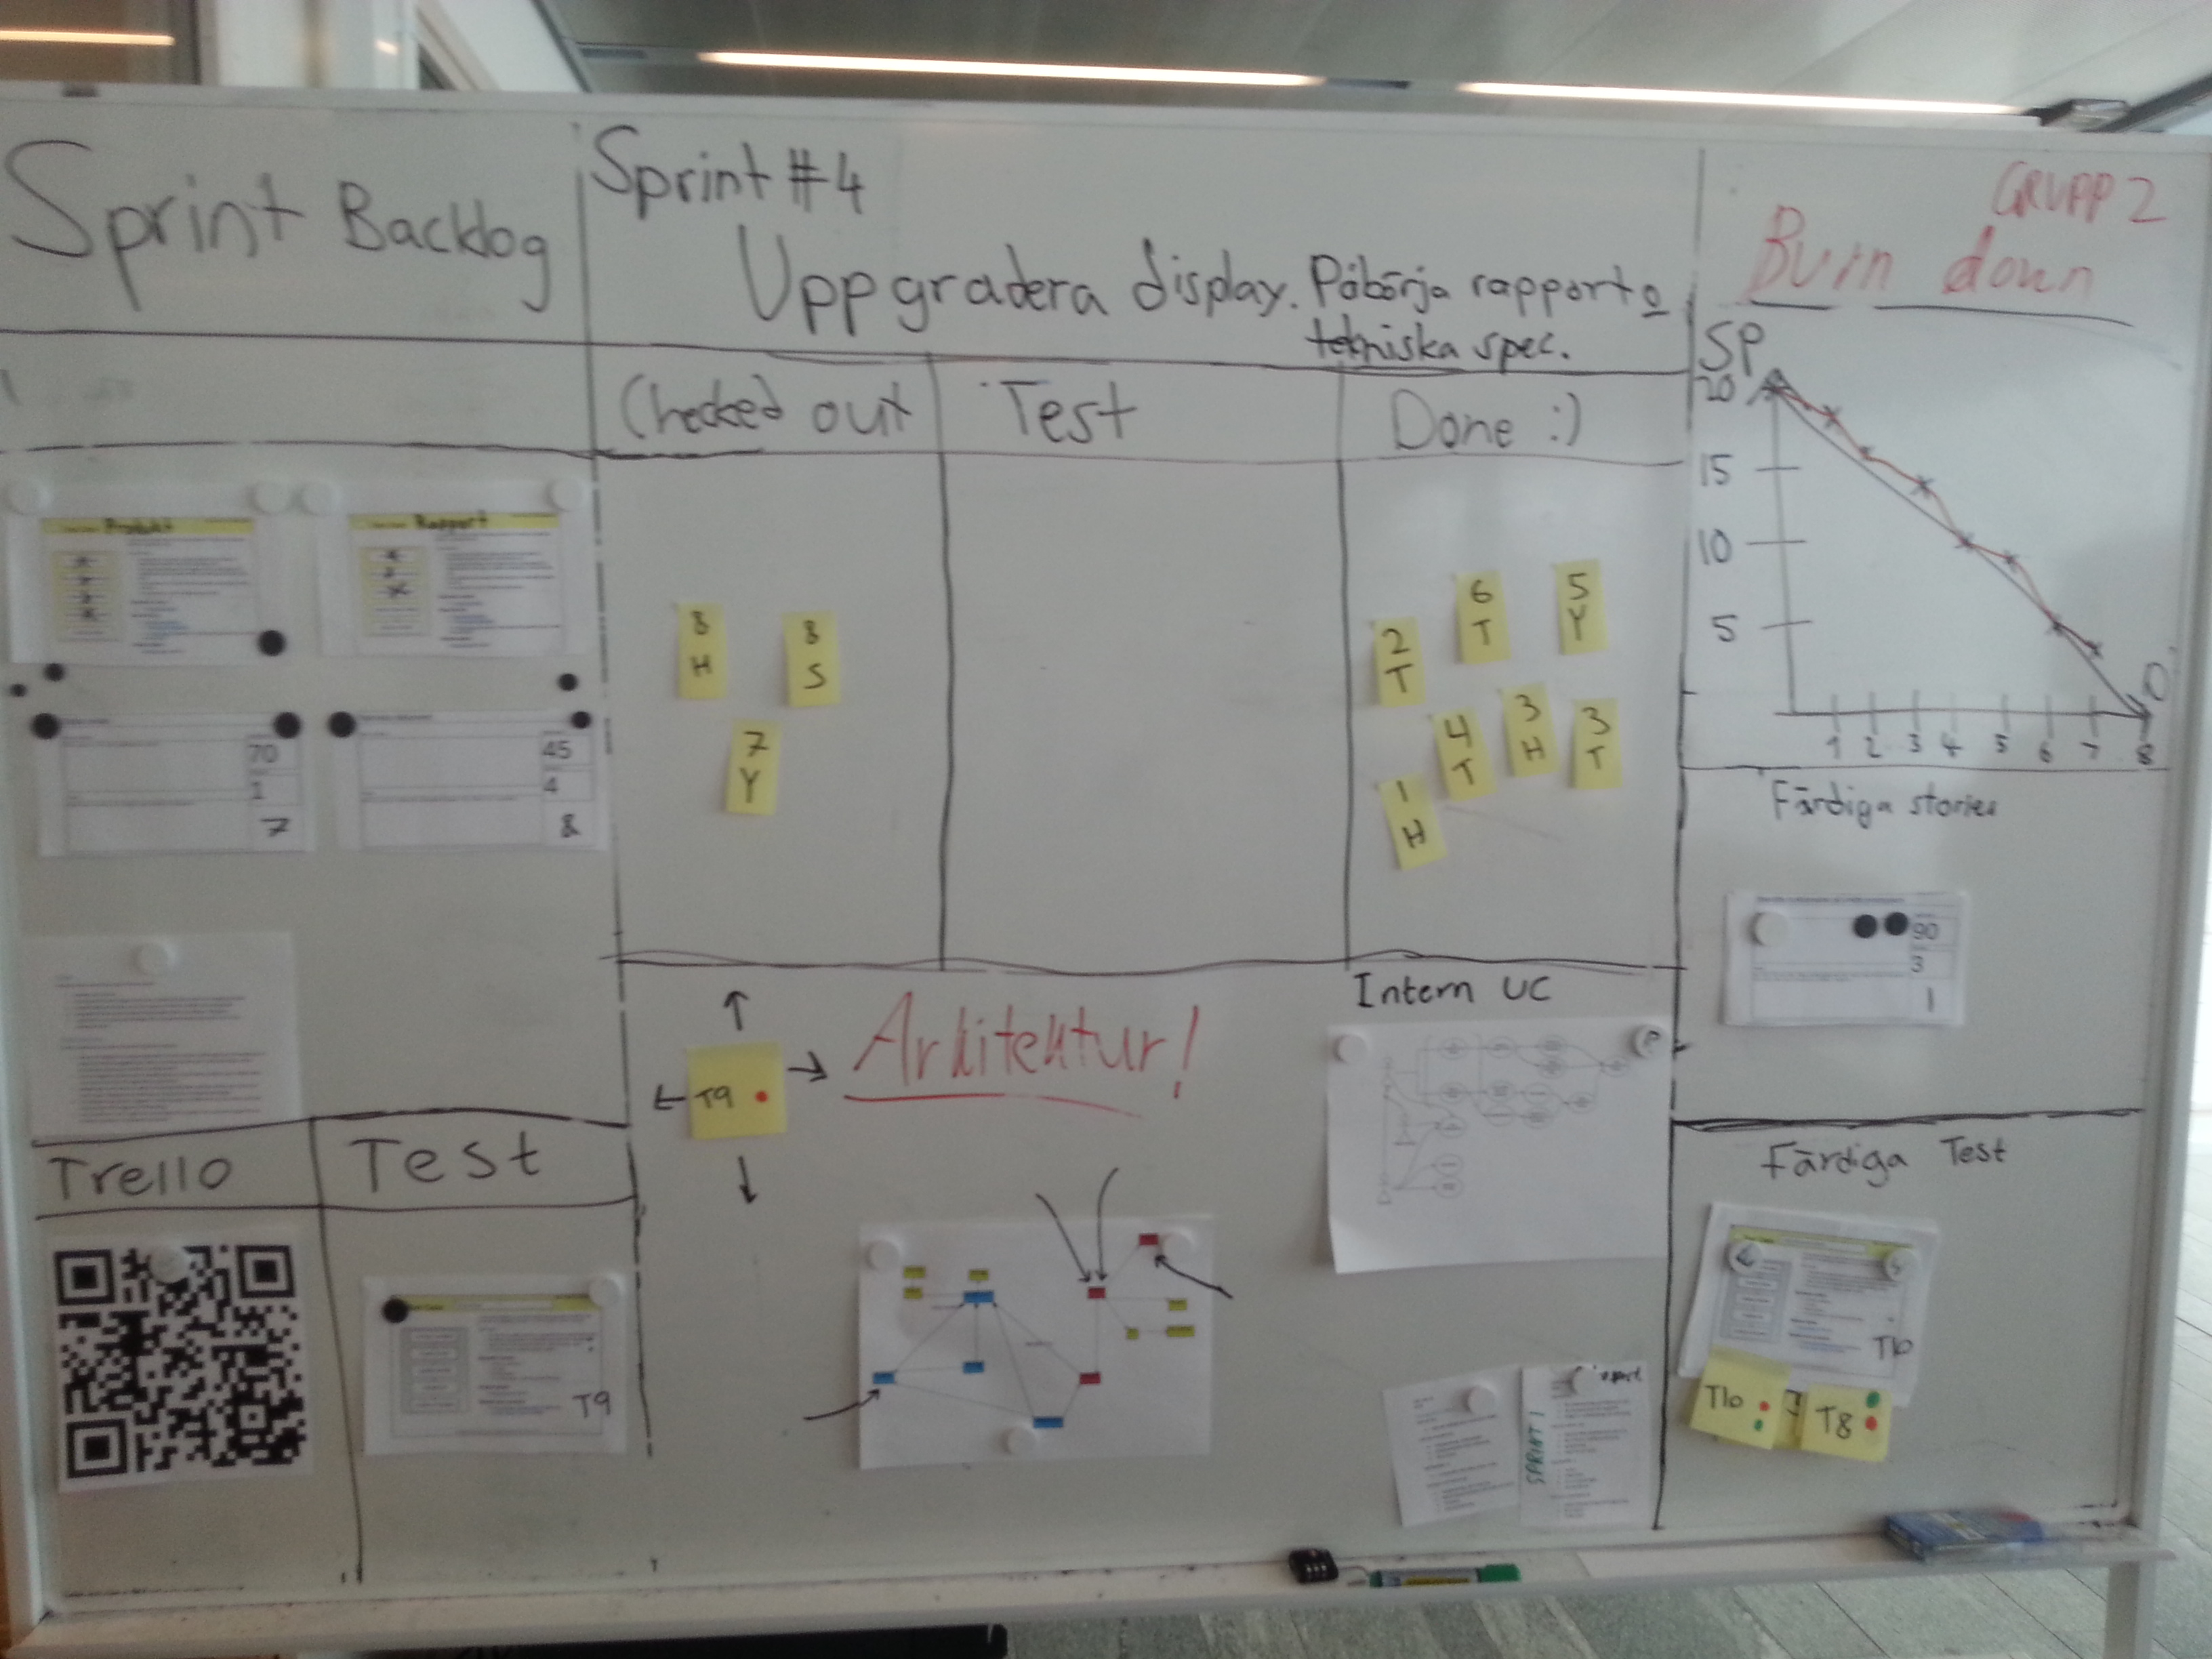
\includegraphics[width=3in]{varsprint}
% where an .eps filename suffix will be assumed under latex,
% and a .pdf suffix will be assumed for pdflatex; or what has been declared
\DeclareGraphicsExtensions.
\caption{Intern sida för projektgruppen (vald ansats).}
\label{varsprint}
\end{figure}

\begin{figure}[H]
\centering
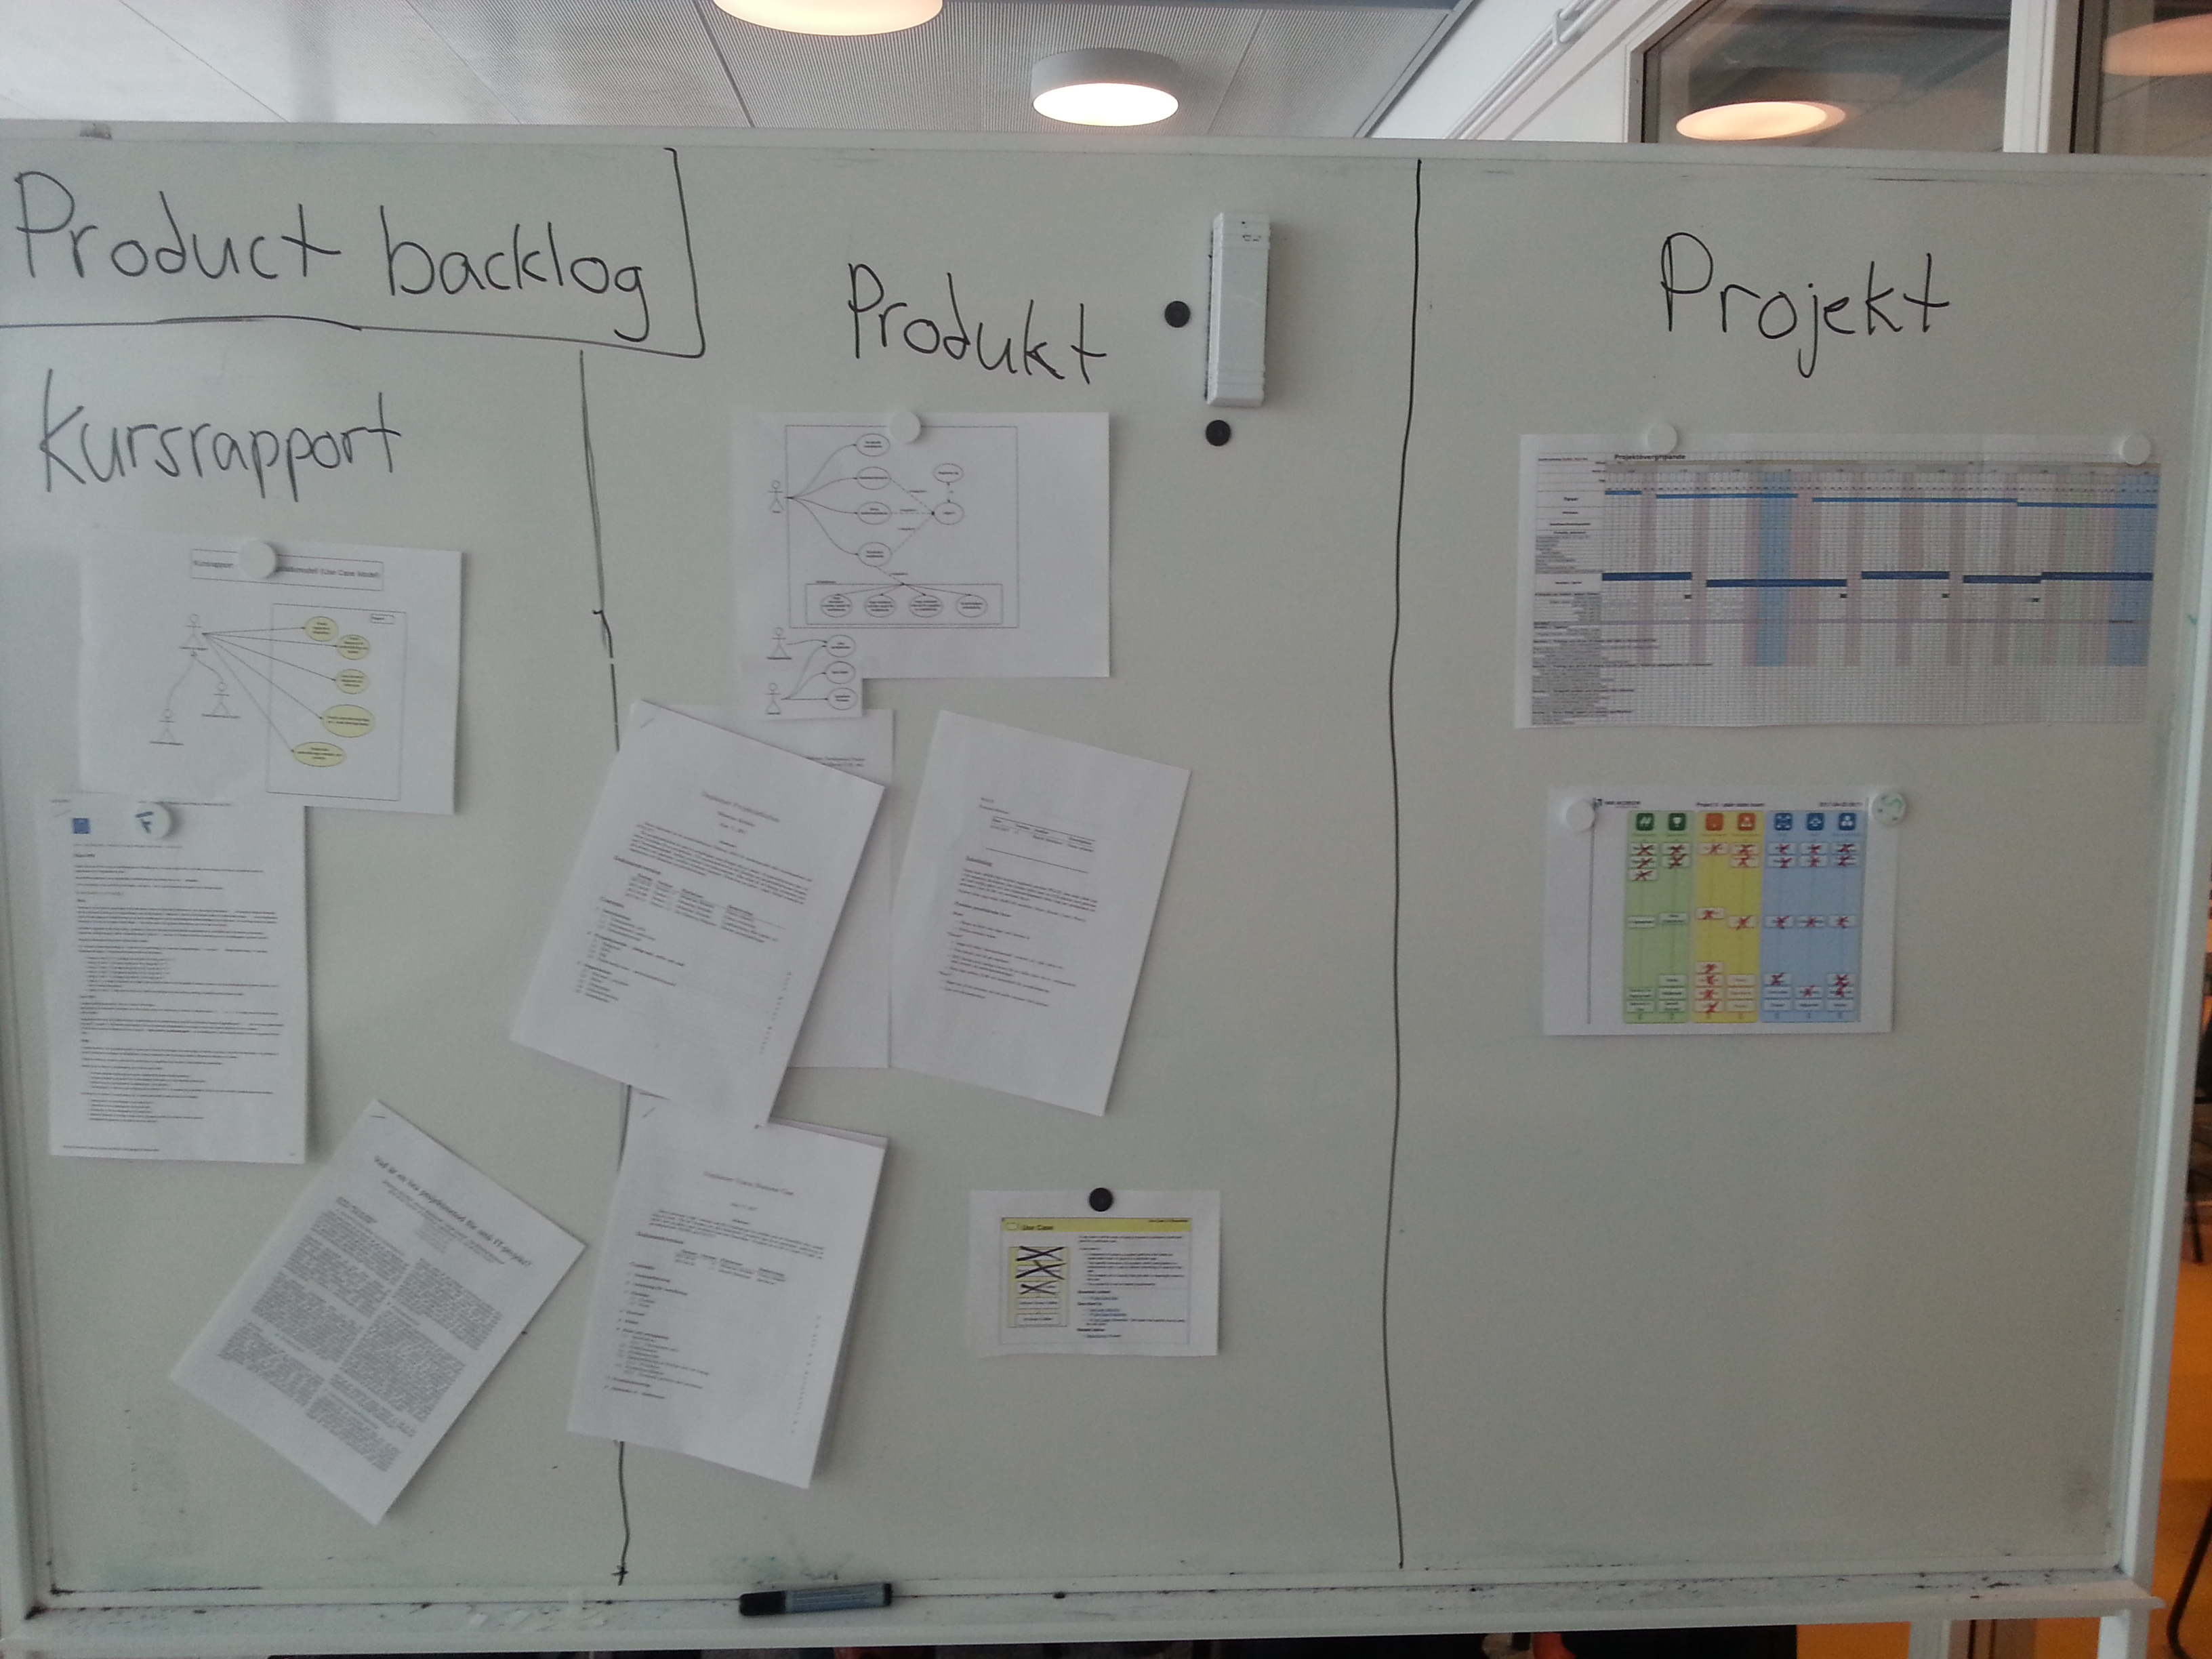
\includegraphics[width=3in]{varproduct}
% where an .eps filename suffix will be assumed under latex,
% and a .pdf suffix will be assumed for pdflatex; or what has been declared
\DeclareGraphicsExtensions.
\caption{Publik sida för projektgruppen (vald ansats) .}
\label{varproduct}
\end{figure}


\subsubsection{Scruminspirerade projektaktiviteter (vald ansats)}



% use section* for acknowledgment
\section{Undersökningsmetoder} \label{sec:under}
Detta kapitel beskriver vilka metoder som använts i undersökningen. Metoderna är valda och specificerade så att de skall kunna ge svar på ett antal följdfrågor som identifierats i denna undersökning. Först anges frågorna och sedan följer metodbeskrivning.
\subsection{Frågor att besvara i undersökningen}

\begin{enumerate}

\item Hur skall man bedöma/redovisa om en delprojektmetod eller praktik är bra?

\item Hur kan man kategorisera, välja, och namnge projektmetoder (projektpraktiker) och (verklighetsbeskrivning) så att diskussionen om dito blir begreppsmässigt konsisten för ingenjörer inom IT-området (s.k. ontologi?).

\item Vilka ansvarsroller skall användas som ansats i projektet?

\item Vad består ett projekt av och vilka metoder/praxis skall användas, undersökas och bedömmas? Vilken ansats skall göras?

\end{enumerate}

\subsection{Metodbeskrivning}
Den centrala metoden i undersökningen är att avgöra om olika valda projekt-praktiker och arbetssätt är ”bra” och om de bidrar till att göra hela projektprocessen bra. Åstadkommer/skapar projektet rätt saker och konstrueras lösningar på bästa sätt?

Metoden för att samla data i denna fråga blir induktiv då erfarenheten i gruppen är ytterst liten. Arbetssättet blir att efterhand som projektet fortskrider så förs bedömningsområden som anses vitala och bedömningskriterier in i en tabell kontinuerligt. Tabellen, se kapitel ”Resultat”, dess innehåll och dess utformning förbättras också hela tiden.\\
\\
\textbf{Metod 1: Undersökningsmetod} se figur. De gula fälten är aktiviteter som kopplar till själva undersökningen. Metoden följer principer för vetenskaplighet enligt Andersson och Ekholm \cite{Andersson02}.

%Exempel på hur man lägger in en bild
\begin{figure}[H]
\centering
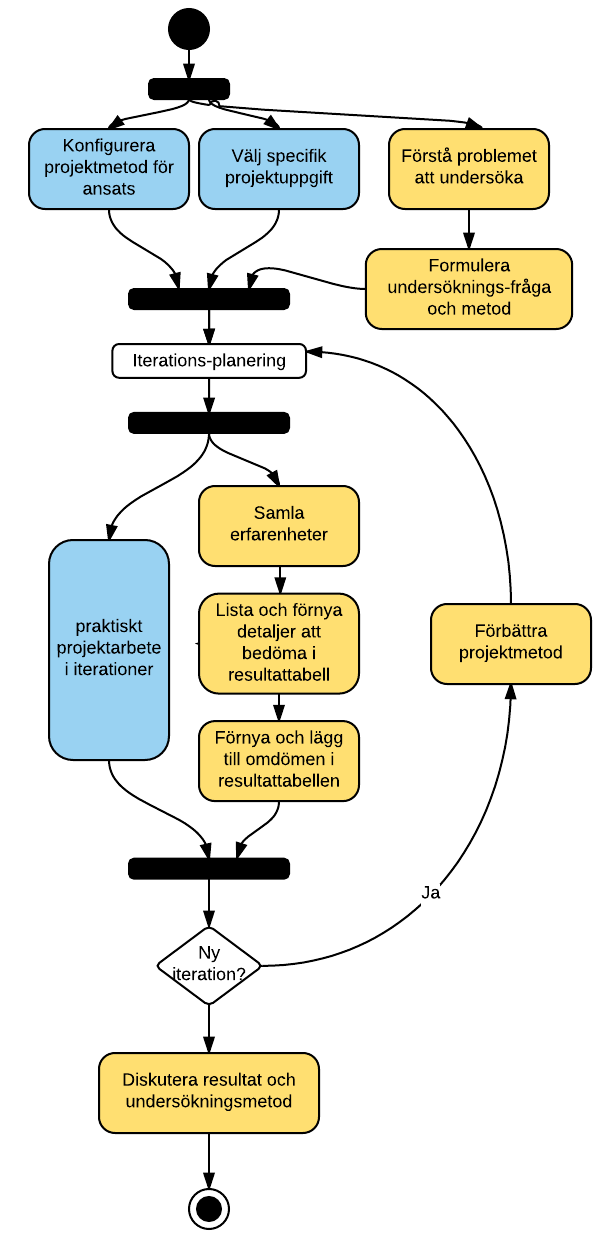
\includegraphics[width=2.5in]{invmethod}
% where an .eps filename suffix will be assumed under latex,
% and a .pdf suffix will be assumed for pdflatex; or what has been declared
\DeclareGraphicsExtensions.
\caption{Undersökningsmetod för ``Vad är en bra projektmetod för små IT-projekt?''.}
\label{undersokningsmetod}
\end{figure}

\textbf{Metod 2: Begrepp} Då det inom detta område saknas en tydlig nomenklatur då många företag och projektgrupper använder samma begrepp med olika betydelse är det viktigt att tydligt definiera rapportens begreppsvärld.

Begrepp som används kommer om möjligt följa OMGs \cite{OMG} standard Essence - Kernel and Language for Software Engineering Methods \cite{Jacobson13}.

Följande bilder listar illustrativt centrala begrepp. I denna artikel kommer de engelska begreppen att fritt översättas till svenska då risken för missförstånd anses liten. se figur \ref{begrepp} och \ref{practice}.

\begin{figure}[H]
\centering
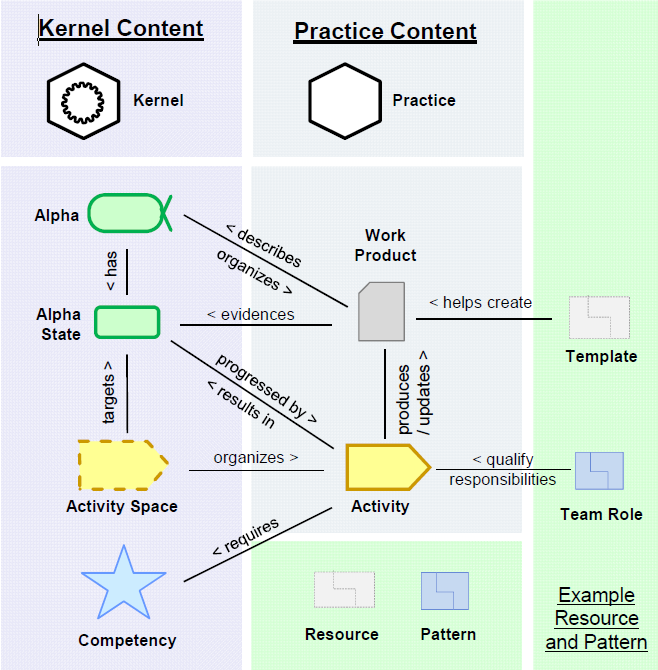
\includegraphics[width=2.5in]{essencebegrepp}
% where an .eps filename suffix will be assumed under latex,
% and a .pdf suffix will be assumed for pdflatex; or what has been declared
\DeclareGraphicsExtensions.
\caption{Begrepp (Elves{\ae}ter, Benguria, \& Ilieva, 2013)}
\label{begrepp}
\end{figure}

\begin{figure}[H]
\centering
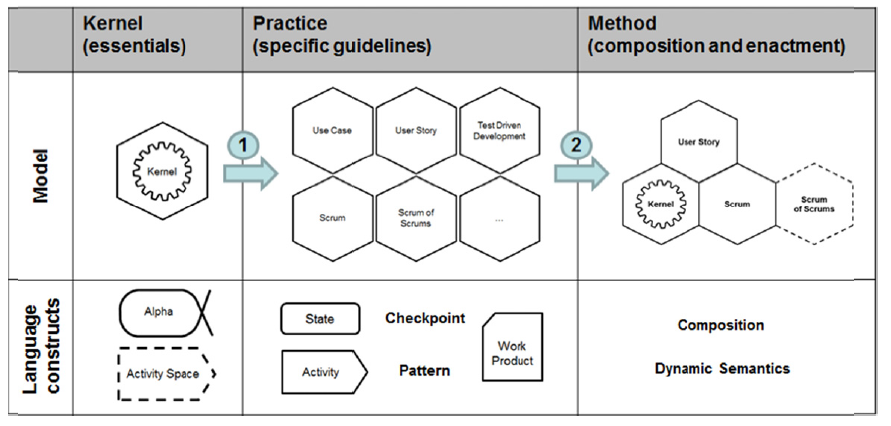
\includegraphics[width=3in]{practice}
% where an .eps filename suffix will be assumed under latex,
% and a .pdf suffix will be assumed for pdflatex; or what has been declared
\DeclareGraphicsExtensions.
\caption{Practice och Methods (Elves{\ae}ter, Striewe, McNeile, \& Berre, 2012)}
\label{practice}
\end{figure}

\section{Genomförande} \label{sec:genom}
I följande kapitel redovisas viktiga beslut, förändringar och anpassningar som gjorts i projektmetod, projektpraktiker, värderingar, beslut mm som gjorts under studiens genomförande.\\
\\
\textbf{NEDAN VISAS GENERELL LAYOUT FÖR DE ENSKILDA DELARNA, SKRIV SOM LÖPANDE TEXT}
\begin{enumerate}
\item Kort om rollen.
\item Vad som provats i rollen
\item Hur det som provades fungerade som metod för "små IT-projekt".
\item Alternativa metoder som kan fungera bättre eller kan provas i framtiden.
\item Lyft fram ett antal bitar från try, keep, skip som har med rollen att göra. Ta fram det bästa och tänk hur det relaterar till rollen och projktmetoder för små IT-projekt.
\item Ta upp allt speciellt bra/dåligt i rollen, verktyg (git), metoder, processer osv.
\item Återkoppla till litteratur och referera.
\end{enumerate}

\subsection{Projektledning (Sebastian Heimlén)}
Projektledarrollen innehåller egentligen två delar - leadership och management. Dessa två delar har i detta projekt slagits ihop och innehas av en person.

Leadership definieras enligt Essence [Referens] som en roll som skall inspirera och motivera projektgruppen för att de på ett framgångsrikt sätt skall kunna genomföra projektet i enlighet med kraven.

Management definieras enligt Essence [Referens] som en administrativ och organiserande roll vars uppgifter är att koordinera, planera samt spåra arbetet i projektet, för att se till rätt saker blir gjorda vid rätt tillfällen för att maximera projektetes chans till framgång.

För att kunna leda en projektgrupp krävs det att projektledaren har koll på målet med projektet, vad som krävs för att nå målet och hur projektgruppen ligger till. Det är viktigt att ha en bra helhetsbild av projektet och en överblick över gruppen så att projektledaren kan ta snabba beslut i de fall där projektet börjar hamna snett. Projektgenomförandet bestod av ett antal iterationer där fokus låg på att hitta en lagom nivå att leda på, planera upp följande iterationer och dess mål och samtidigt stödja och vara en bidragande faktor i arbetet att producera produkten. De prövade ansatserna som utvärderats i projektet är:

\begin{itemize}
\item Projektdefinition (Eklund \cite[s. 137-146]{Eklund14})
\item Projekt/iterationsplan Gantt
\item Scrum (Kniberg \cite{Kniberg07})
  \begin{itemize}
    \item ``Scrumboard''
	  \item ``Stories''
    \item ``Tech Stories''
    \item ``Story points''
    \item ``Backlog''
\end{itemize}
\item Use-Case 2.0 (Jacobson \cite{Jacobson11})
	\begin{itemize}
	\item ``Use-Case''
  \item ``Use-Case Slice''
  \end{itemize}
\item KanBan (Kniberg \cite{Kniberg10})
\end{itemize}

\noindent \textbf{Projektdefinition och projektplan}\\
\\
Det första som skedde i början av projektet var att projektdefinition och projektplan skrevs, helt i enlighet med Eklund \cite[s. 138-139]{Eklund14} och Sommerville \cite[s. 619]{Sommerville10} som bägge poängterar värdet av att i starten av projektet göra en grovplan över projektets olika delar, då det är av största vikt som projektledare att planera upp projektet. Undersökningsmetodens första och andra cykel visade att denna ansats spelade en vital i att hålla projektet strukturerat och projektplanen har kontinuerligt uppdaterats och manipulerats därefter, för att möta skiftande krav och oförutsedda problem. Projektdefinition och projektplan följer i stora drag den föreslagna ansatsen.\\
\\
\textbf{Scrum, use case och stories}\\
\\
I de två första iterationerna nyttjade gruppen Scrum i kombination med stories, story points, burn down chart och tasks som Kniberg \cite{Kniberg07} förespråkat. Undersökningsmetodens första och andra cykel visade att detta fungerade bra, men att det var något svårt att koppla uppgifter till användarkrav och det blev lite väl mycket ad-hoc. I början av sprint tre blev gruppen introducerad till Jacobsons use-cases \cite{Jacobson11}. Fördelar sågs i båda metoder men use-cases gav mer kontroll då de gick att dela upp i slices på ett strukturerat sätt och då skapa tillräckligt små arbetsuppgifter som gick att lösa inom en iteration, och därför prövades use-case metoden tillsammans med stories i iteration tre. I samband med detta så började ett närmare sammarbete mellan projektledare och kravansvarig då båda parter arbetade med use-cases, men på olika sätt. Projektledare för att organisera arbetet och kravansvarig för att fånga krav. Detta samarbete rönte framgång och i undersökningscykel tre och fyra visade det sig att gruppen arbetat sig igenom fler storypoints än i de tidigare iterationerna, även fast arbetstiden var kortare.

En stor anledning till detta tros vara det konkreta samarbetet mellan projektledare och kravansvarig, och detta gjordes möjligt tack vare att båda parter använde use-cases till sitt förfogande. Denna konstellation av metoder illät projektgruppen att fortsätta jobba med stories, story points, burn down charts och tasks, men även integrera Essence \cite{Jacobson13} i form av use-cases i arbetet och på så ha en tydlig standard att stå på.

De uppgifter som ej gick att koppla till något användarkrav, till exempel overhead från kursen, lades i så kallade ``tech-stories''. Undersökningen visade att detta är ett bra sätt att hantera overhead, dock är det ett illa men, då en helst undviker uppgifter som ej verkar mot kundens krav.

\subsection{Arkitekt (Teo Klestrup Röijezon)}
Arkitektrollen handlar om att analysera kundens krav, och att sedan kunna bygga en
bred teknisk plan som uppfyller dem. Denna roll handlar dock inte om hur varje
komponent fungerar internt, utan snarare om hur de samarbetar och tillsammans
uppfyller kraven.

Utifrån kundrepresentatens krav delade jag upp lösningen i olika komponenter
med respektive ansvarsfördelning och ritade ett arkitekturdiagram (se Figur
\ref{architecture-logical}). Sedan reviderades arkitekturen vid behov mellan
varje sprint. Diagrammet är baserat på den logiska modellen från
``4+1-metoden''\cite{Kruchten95}, men använder vanlig UML-notation, och innehåller
även viss information uppdelningen mellan fysiska maskiner, samt om våran
ansvarsfördelning (genom färgkodning).

\begin{figure}[H]
\centering
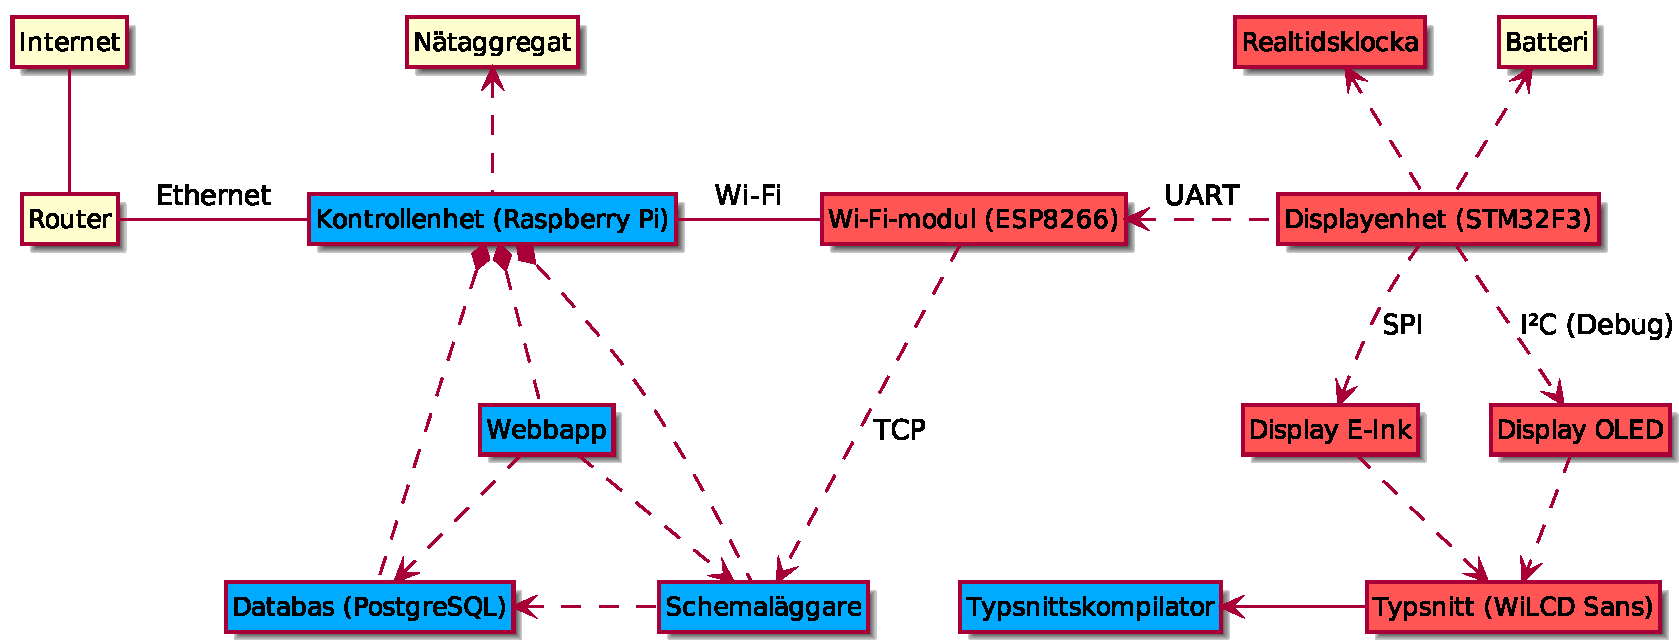
\includegraphics[width=9cm]{../../Arkitektur/Arkitektur-eps-converted-to.pdf}
\caption{Vår Logiska Arkitektur}
\label{architecture-logical}
\end{figure}

En annan inspirationskälla har varit Anders Sjögrens exempel (se
\ref{architecture-logical-sjoegren}), men jämfört med det så har våran
modell färre detaljer om komponenterna är implementerade, eftersom vi
ansåg att det skulle bli för komplicerat, speciellt med tanke på spridningen
av våra komponenter.

\begin{figure}[H]
\centering
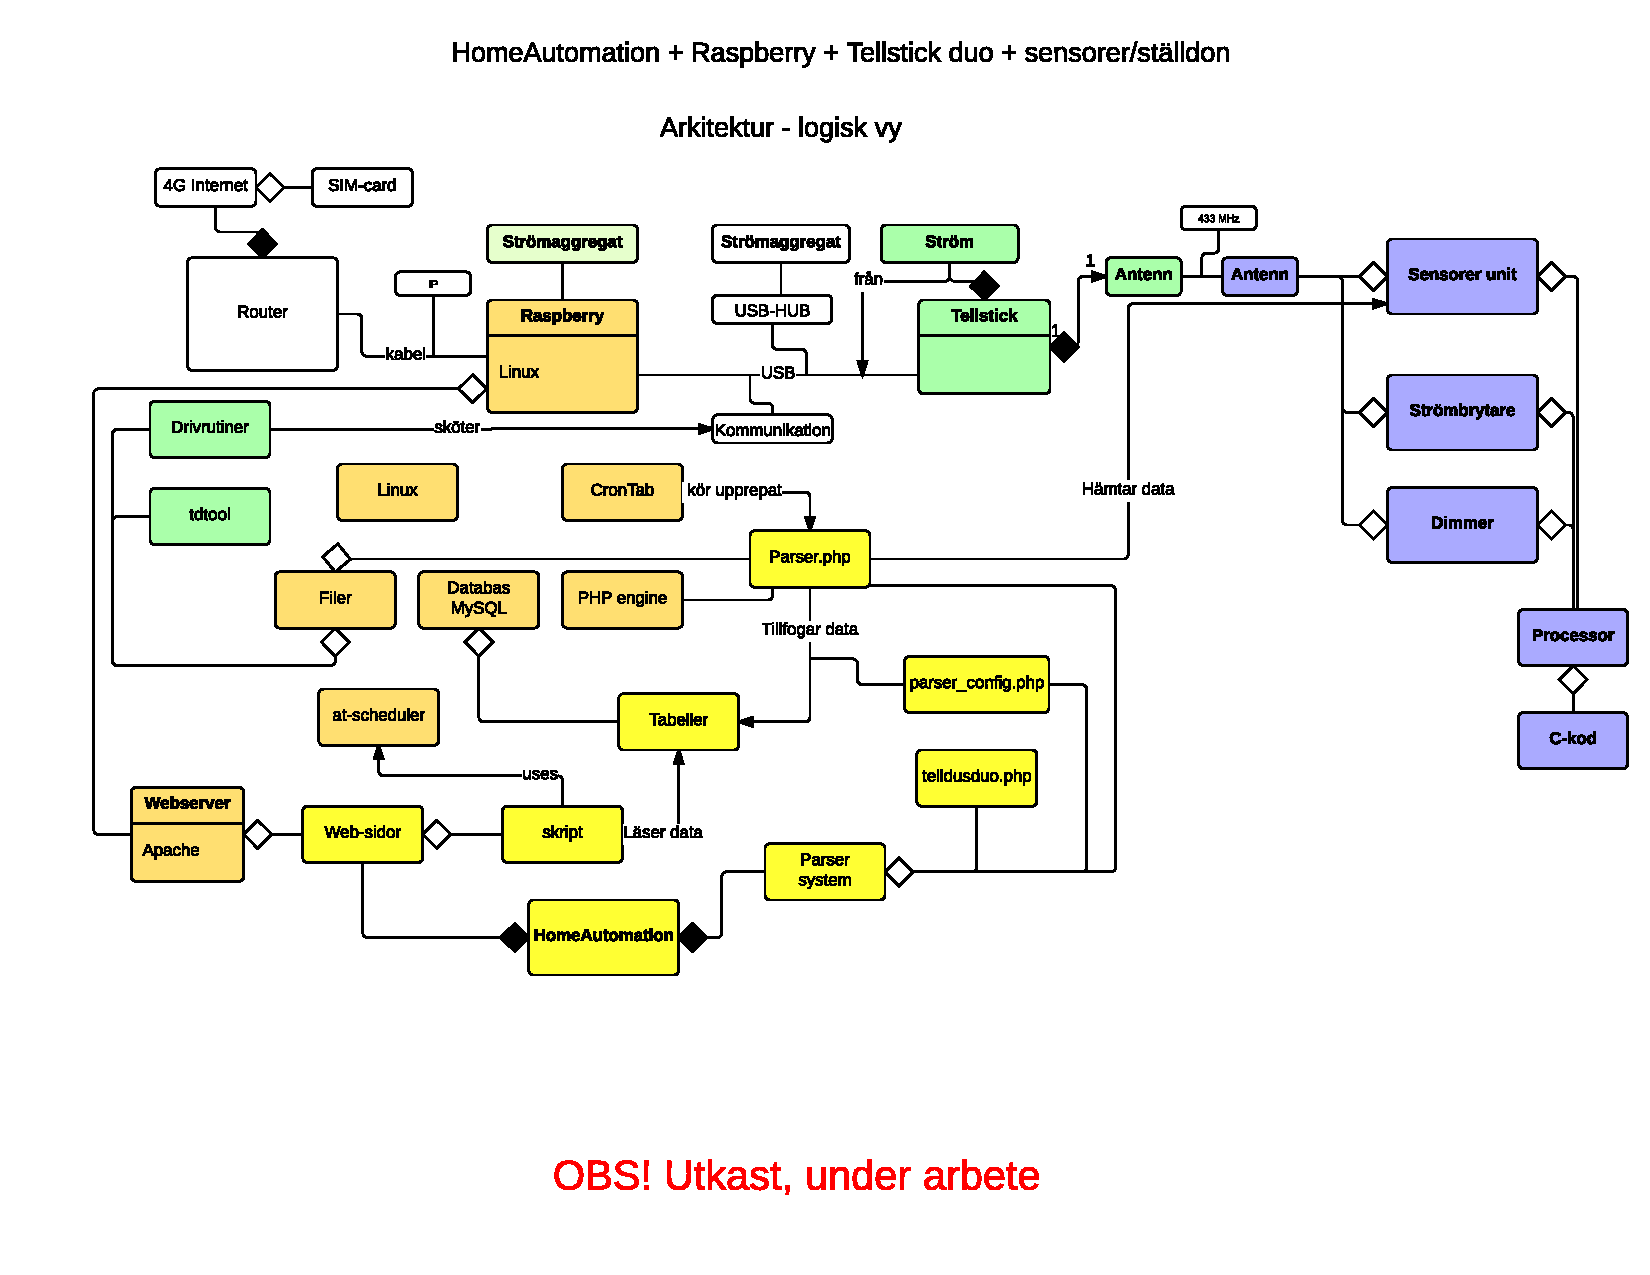
\includegraphics[width=9cm]{homeautomation-logisk}
\caption{Anders Sjögrens Exempel på Logisk Arkitektur\cite{SjoegrenHALogisk}}
\label{architecture-logical-sjoegren}
\end{figure}

I stället flyttades dessa detaljer till separata diagram per komponent, exempelvis
modellererar Figur \ref{architecture-webside-class} våran webbsida utifrån
Jim Conallens system\cite{Conallen99}.

\begin{figure}[H]
\centering
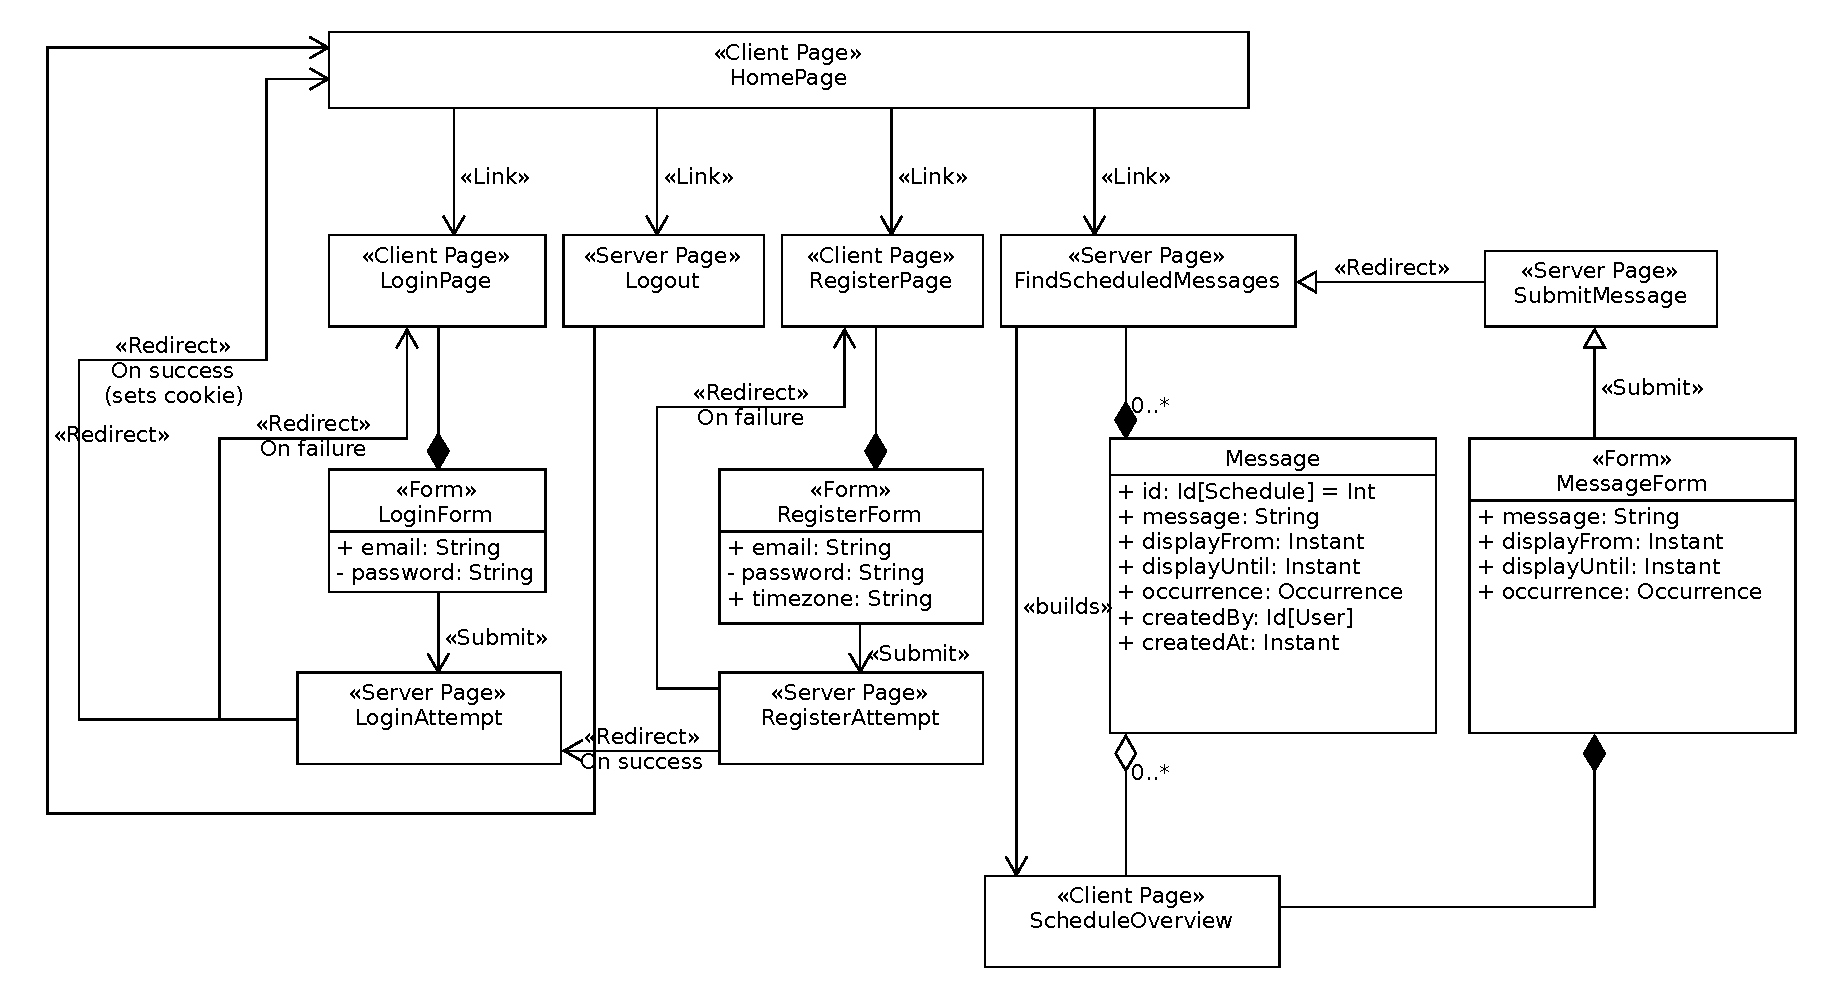
\includegraphics[width=9cm]{../../Arkitektur/Webbsida_UML.pdf}
\caption{Arkitektur För Webbsidan}
\label{architecture-webside-class}
\end{figure}

Våran arkitektur har varit relativt konsekvent under projektet, förutom att den
från början inte visade att vi behövde utveckla ett typsnitt, samt att vi inte
hade räknat med att byta skärm.

För framtida projekt så anser jag att den övergripande arkitekturen fungerade bra,
och var lagom detaljerad, men att de detaljerade diagrammen (exempelvis för webbsidan)
inte hade ett stort extra värde över själva koden utan bara tillförde ännu ett dokument
att uppdatera vid ändringar. Dock varierar värdet självklart beroende på gruppens storlek.

Dessutom verkar inte Conallens system\cite{Conallen99} välanpassat för moderna, mer dynamiska,
sidor, men det har inte varit ett problem i vårat fall. 

Ett annat mindre problem har varit att vi har varierat mycket mellan olika modelleringsverktyg.
Från början använde jag Umbrello\cite{Umbrello} eftersom det var integrerat i KDE, men gick efter
en del frustration över till UMLet\cite{UMLet}, före jag till slut började använda
PlantUML\cite{PlantUML} eftersom den använder ett textbaserat format som är enkelt för människor att ändra.

Dessa övergångar visade tyvärr att standardiseringen mellan dessa verktyg är, snällt sagt, dålig,
vilket innebar att varje övergång gav ett val mellan att göra om alla diagram för hand, eller att
ha dokumentationen utspridd i ännu ett filformat.

\subsection{Kundrepresentant}

\subsection{Testansvarig}

\section{Resultat} \label{sec:res}
Nedan listas de punkter som ska behållas (Keep), testas (Try) och som har varit problem (Problem), de har sammanställts utifrån de retrospektivmöten som gruppen har hållit i slutet av varje sprint. 

De innehåller även förslag på förbättringar som kan implementeras i framtida projekt samt idéer som kan tänkas komma till nytta både för att förbättra framtida projekt och undvika problem.

\begin{table}[H]
	\small
  \centering
	\begin{tabular}{|p{1.5cm}|p{2.3cm}|p{1.5cm}|p{1.5cm}|} % to \columnwidth {"X[l]"X[l]"X[l]"l|}
    \hline
    Keep & Motivation & Förbättringar & Referenser \TBstrut \\
    \hline
    Scrum-metodik  & Scrum organiserar IT-arbete på ett sätt som passar många utvecklare och beställare. Den iterativa processen tillåter kontinuerlig utvärdering. Scrum ger även ett arbetssätt som inte är toppstyrt och lämpar sig väl i små projekt  & & Kniberg \cite{Kniberg07} \TBstrut \\
    \hline
    Modiferad Kanban tavla & Ger en tydlig bild över hur arbetet fortlöper, då varje task kan följas från "Checked out" till "Done" & Eventuellt kan det läggas till plats för sätta tasks som den ansvarige behöver hjälp med & Sommerville \cite{Sommerville10}, Kniberg \cite{Kniberg10} \TBstrut \\
    \hline
    Virtuell tavla & Övergången till en virtuell tavla, i Trello, skapade en lättare platform för att planera och ha kontroll över projektet. Då det inte gick att vara på plats vid den fysiska tavlan alltid. & Integrera en fysisk tavla med den virtuella, kanske via en projekt eller annan utrustning & \TBstrut \\
    \hline
    User stories, User slices, User tasks & User stories hjälpte att skapa en tydlig struktur i arbetet, hur de olika delarna av systemet hängde ihop  & I små projekt fungerade det bra att endast ha en övergripande Story, och få antal slices, för att i ställe fokusera på små tasks, 1-3 Story points långa. & Jacobson \cite{Jacobson11} \TBstrut \\
    \hline
    Budgetering av story points & Genom att arbeta med små tasks, gav det oss möjligheten att precis budgetera att ungefär hur lång tid varje del skulle ta. Detta hjälpte oss att få en stadig burndown som visade hur projektet gick&  & \TBstrut \\
    \hline
    Trello & Som en virtuell platform fungerade Trello bra, både för lägga upp tasks och test& Viss förbättring att involvera User slices i Trello kunde ha implementerats  & \TBstrut \\
    \hline
  \end{tabular}
\end{table}

\begin{table}[H]
	\small
  \centering
	\begin{tabular}{|p{1.9cm}|p{2cm}|p{1.7cm}|p{1.2cm}|} % to \columnwidth {"X[l]"X[l]"X[l]"l|}
    \hline
    Try & Try what? & Motiveringar & Referenser \TBstrut \\
    \hline
    Riskbedömning & Ökad riskbedömning inklusive alternativ om en bit av systemet skulle visas ej fungera till sprintens slut. & För att skapa ett stabilt projekt som kan hantera motgångar bättre& \TBstrut \\
    \hline
    Automatiserade tester & Automatisera de tester som går. & Detta för att minska belastningen på testansvarig& \TBstrut \\
    \hline

  \end{tabular}
\end{table}

\begin{table}[H]
	\small
  \centering
	\begin{tabular}{|p{1.9cm}|p{1.7cm}|p{2.2cm}|p{1.2cm}|} % to \columnwidth {"X[l]"X[l]"X[l]"l|}
    \hline
    Problem & Skip or replace what? & Motiveringar & Referenser \TBstrut \\
    \hline
    Riskbedömning & Skapa alternativa idéer om problem skulle uppstå &  Riskbedömningen har under projektet inte jämt haft någon handlingsplan om problem skulle ha dykt upp& \TBstrut \\
    \hline
    Teststrukturer &Skapa tydlig teststruktur tidigt i projektet &Teststrukturen under de första sprintarna var inte så genom arbetad och utvecklad, men blev under sista sprinten bättre.  & \TBstrut \\
    \hline

  \end{tabular}
\end{table}

\section{Analys / Förbättringsförslag} \label{sec:analys}

\section{Diskussion} \label{sec:disk}

\subsection{Metoddiskussion}

\subsection{Resultatdiskussion}

\subsection{Bidrag till vetenskaplighet, ingenjörserfarenhet (studenterfarenhet?)}

\section{Slutord} \label{sec:slutord}

% trigger a \newpage just before the given reference
% number - used to balance the columns on the last page
% adjust value as needed - may need to be readjusted if
% the document is modified later
%\IEEEtriggeratref{8}
% The "triggered" command can be changed if desired:
%\IEEEtriggercmd{\enlargethispage{-5in}}

% references section

% can use a bibliography generated by BibTeX as a .bbl file
% BibTeX documentation can be easily obtained at:
% http://mirror.ctan.org/biblio/bibtex/contrib/doc/
% The IEEEtran BibTeX style support page is at:
% http://www.michaelshell.org/tex/ieeetran/bibtex/
%\bibliographystyle{IEEEtran}
% argument is your BibTeX string definitions and bibliography database(s)
%\bibliography{IEEEabrv,../bib/paper}
%
% <OR> manually copy in the resultant .bbl file
% set second argument of \begin to the number of references
% (used to reserve space for the reference number labels box)
%\begin{thebibliography}{1}

%\bibitem{IEEEhowto:kopka}
%H.~Kopka and P.~W. Daly, \emph{A Guide to \LaTeX}, 3rd~ed.\hskip 1em plus
%  0.5em minus 0.4em\relax Harlow, England: Addison-Wesley, 1999.

%\bibitem{}

%\end{thebibliography}

\bibliographystyle{IEEEtran}
\bibliography{sources}

\appendices
\section{Personliga resultat}

\subsection{Kundrepresentant (Henrik Björklund)}
\begin{table}[H]
	\small
  \centering
	\begin{tabular}{|p{1.5cm}|p{2cm}|p{1.8cm}|p{1.5cm}|} % to \columnwidth {"X[l]"X[l]"X[l]"l|}
    \hline
    Keep & Motivation & Förbättringar & Referenser \TBstrut \\
    \hline
    Use-Cases \& Slices & Use-Cases är fångar in krav på ett intuitiv & & \TBstrut \\
    \hline
    Scrum & Scrum organiserar IT-arbete på ett sätt som passar många utvecklare och beställare. Den iterativa processen tillåter kontinuerlig utvär & & \TBstrut \\
    \hline
    Projekttavla & Projekttavlan fungerar som en tydlig & & \TBstrut \\
    \hline
  \end{tabular}
\end{table}

\begin{table}[H]
	\small
  \centering
	\begin{tabular}{|p{1.5cm}|p{2cm}|p{1.8cm}|p{1.5cm}|} % to \columnwidth {"X[l]"X[l]"X[l]"l|}
    \hline
    Problem & Try what? & Motiveringar & Referenser \TBstrut \\
    \hline
    Use-Cases \& Slices & Use-Cases är fångar in krav på ett intuitiv & & \TBstrut \\
    \hline
    Scrum & Scrum organiserar IT-arbete på ett sätt som passar många utvecklare och beställare. Den iterativa processen tillåter kontinuerlig utvär & & \TBstrut \\
    \hline
    Projekttavla & Projekttavlan fungerar som en tydlig & & \TBstrut \\
    \hline
  \end{tabular}
\end{table}

\begin{table}[H]
	\small
  \centering
	\begin{tabular}{|p{1.5cm}|p{2cm}|p{1.8cm}|p{1.5cm}|} % to \columnwidth {"X[l]"X[l]"X[l]"l|}
    \hline
    Problem & Skip or replace what? & Motiveringar & Referenser \TBstrut \\
    \hline
    Use-Cases \& Slices & Use-Cases är fångar in krav på ett intuitiv & & \TBstrut \\
    \hline
    Scrum & Scrum organiserar IT-arbete på ett sätt som passar många utvecklare och beställare. Den iterativa processen tillåter kontinuerlig utvär & & \TBstrut \\
    \hline
    Projekttavla & Projekttavlan fungerar som en tydlig & & \TBstrut \\
    \hline
  \end{tabular}
\end{table}

\subsection{Arkitekt (Teo Klestrup Röijezon)}
\begin{table}[H]
	\small
  \centering
	\begin{tabular}{|p{1.5cm}|p{2cm}|p{1.8cm}|p{1.5cm}|} % to \columnwidth {"X[l]"X[l]"X[l]"l|}
    \hline
    Keep & Motivation & Förbättringar & Referenser \TBstrut \\
    \hline
    Use-Cases \& Slices & Use-Cases är fångar in krav på ett intuitiv & & \TBstrut \\
    \hline
    Scrum & Scrum organiserar IT-arbete på ett sätt som passar många utvecklare och beställare. Den iterativa processen tillåter kontinuerlig utvär & & \TBstrut \\
    \hline
    Projekttavla & Projekttavlan fungerar som en tydlig & & \TBstrut \\
    \hline
  \end{tabular}
\end{table}

\begin{table}[H]
	\small
  \centering
	\begin{tabular}{|p{1.5cm}|p{2cm}|p{1.8cm}|p{1.5cm}|} % to \columnwidth {"X[l]"X[l]"X[l]"l|}
    \hline
    Problem & Try what? & Motiveringar & Referenser \TBstrut \\
    \hline
    Use-Cases \& Slices & Use-Cases är fångar in krav på ett intuitiv & & \TBstrut \\
    \hline
    Scrum & Scrum organiserar IT-arbete på ett sätt som passar många utvecklare och beställare. Den iterativa processen tillåter kontinuerlig utvär & & \TBstrut \\
    \hline
    Projekttavla & Projekttavlan fungerar som en tydlig & & \TBstrut \\
    \hline
  \end{tabular}
\end{table}

\begin{table}[H]
	\small
  \centering
	\begin{tabular}{|p{1.5cm}|p{2cm}|p{1.8cm}|p{1.5cm}|} % to \columnwidth {"X[l]"X[l]"X[l]"l|}
    \hline
    Problem & Skip or replace what? & Motiveringar & Referenser \TBstrut \\
    \hline
    Use-Cases \& Slices & Use-Cases är fångar in krav på ett intuitiv & & \TBstrut \\
    \hline
    Scrum & Scrum organiserar IT-arbete på ett sätt som passar många utvecklare och beställare. Den iterativa processen tillåter kontinuerlig utvär & & \TBstrut \\
    \hline
    Projekttavla & Projekttavlan fungerar som en tydlig & & \TBstrut \\
    \hline
  \end{tabular}
\end{table}


\subsection{Testare (Yobart Amino)}
\begin{table}[H]
	\small
  \centering
	\begin{tabular}{|p{1.5cm}|p{2cm}|p{1.8cm}|p{1.5cm}|} % to \columnwidth {"X[l]"X[l]"X[l]"l|}
    \hline
    Keep & Motivation & Förbättringar & Referenser \TBstrut \\
    \hline
    Use-Cases \& Slices & Use-Cases är fångar in krav på ett intuitiv & & \TBstrut \\
    \hline
    Scrum & Scrum organiserar IT-arbete på ett sätt som passar många utvecklare och beställare. Den iterativa processen tillåter kontinuerlig utvär & & \TBstrut \\
    \hline
    Projekttavla & Projekttavlan fungerar som en tydlig & & \TBstrut \\
    \hline
  \end{tabular}
\end{table}

\begin{table}[H]
	\small
  \centering
	\begin{tabular}{|p{1.5cm}|p{2cm}|p{1.8cm}|p{1.5cm}|} % to \columnwidth {"X[l]"X[l]"X[l]"l|}
    \hline
    Problem & Try what? & Motiveringar & Referenser \TBstrut \\
    \hline
    Use-Cases \& Slices & Use-Cases är fångar in krav på ett intuitiv & & \TBstrut \\
    \hline
    Scrum & Scrum organiserar IT-arbete på ett sätt som passar många utvecklare och beställare. Den iterativa processen tillåter kontinuerlig utvär & & \TBstrut \\
    \hline
    Projekttavla & Projekttavlan fungerar som en tydlig & & \TBstrut \\
    \hline
  \end{tabular}
\end{table}

\begin{table}[H]
	\small
  \centering
	\begin{tabular}{|p{1.5cm}|p{2cm}|p{1.8cm}|p{1.5cm}|} % to \columnwidth {"X[l]"X[l]"X[l]"l|}
    \hline
    Problem & Skip or replace what? & Motiveringar & Referenser \TBstrut \\
    \hline
    Use-Cases \& Slices & Use-Cases är fångar in krav på ett intuitiv & & \TBstrut \\
    \hline
    Scrum & Scrum organiserar IT-arbete på ett sätt som passar många utvecklare och beställare. Den iterativa processen tillåter kontinuerlig utvär & & \TBstrut \\
    \hline
    Projekttavla & Projekttavlan fungerar som en tydlig & & \TBstrut \\
    \hline
  \end{tabular}
\end{table}

\subsection{Keep, Try, Skip - Ledning och Styrning (Sebastian Heimlén)}

Denna bilaga tar upp resultat som jag i min roll som projektledare tagit fram under undersökningen. Resultaten kommer främst att handla om delar av projektet som är specifika för min roll, men även lite mer allmäna delar kring IT-projekt som utvecklas med hjälp av dessa projektmetoder som vi använt/utvärderat.

\textbf{1) Iteration 1}

\begin{table}[H]
	\small
  \centering
	\begin{tabular}{|p{1.5cm}|p{2cm}|p{1.8cm}|p{1.5cm}|} % to \columnwidth {"X[l]"X[l]"X[l]"l|}
    \hline
    Keep & Motivation & Förbättringar & Referenser \TBstrut \\
    \hline
  \end{tabular}
\end{table}

\begin{table}[H]
	\small
  \centering
	\begin{tabular}{|p{1.5cm}|p{2cm}|p{1.8cm}|p{1.5cm}|} % to \columnwidth {"X[l]"X[l]"X[l]"l|}
    \hline
    Problem & Try what? & Motiveringar & Referenser \TBstrut \\
    \hline
    Det finns ingen projektplan eller projektdefinition. & Börja planera upp projektet genom att skapa en projektplan och skriv en projektdefinition. & En grovplan över projektet är vitalt för att projektet skall kunna fortlöpa inom ramarna för Eklunds åtagandetriangel. & \cite[s. 128]{Eklund14}, \cite[s. 72]{Sommerville10} \TBstrut \\
    \hline
    Gruppen har precis träffats, och vet ej hur de andra medlemmarna jobbar och/eller hur ambitiösa de är. & Försök lära känna varandra lite, känna av hur de olika medlemmarna jobbar och deras styrkor och svagheter. & Gruppdynamik och moral är väldigt viktigt i projektgrupper, speciellt tidigt i projektet då det annars finns risk att sprickor i gruppen är fördärvliga för hela projektet. & \cite[kap. 7]{Eklund14}. \TBstrut \\
    \hline
    Oklart hur hårt en måste leda. & Lite som förra punkten, jag måste känna av hur självständiga och ambitiösa gruppen är, för att på så sätt se hur hårt jag måste hålla i tyglarna. & En projektledare brukar oftast inte finnas i en projektgrupp som jobbar med Scrum, då tanken med Scrum är att samtliga medlemmar ska kunna agera lite ledare och tillsammans fatta beslut som gynnar gruppen, det är därför viktigt att inte gå in för hårt i ledarrollen, men samtidigt leda tillräckligt hårt så att inte medlemmar slutar att jobba, detta är väldigt beroende på vilken typ av grupp som projektet består av. & \cite[s. 73-74]{Sommerville10}. \TBstrut \\
    \hline
  \end{tabular}
\end{table}

\begin{table}[H]
	\small
  \centering
	\begin{tabular}{|p{1.5cm}|p{2cm}|p{1.8cm}|p{1.5cm}|} % to \columnwidth {"X[l]"X[l]"X[l]"l|}
    \hline
    Problem & Skip or replace what? & Motiveringar & Referenser \TBstrut \\
    \hline
  \end{tabular}
\end{table}

\textbf{Iteration 2}


\begin{table}[H]
	\small
  \centering
	\begin{tabular}{|p{1.5cm}|p{2cm}|p{1.8cm}|p{1.5cm}|} % to \columnwidth {"X[l]"X[l]"X[l]"l|}
    \hline
    Keep & Motivation & Förbättringar & Referenser \TBstrut \\
    \hline
    Den goda grupp- och arbetsmoralen & Arbetet har gått väldigt bra och gruppen kommer bra överrens och jobbar bra tillsammans. En bra arbetsmoral är väldigt viktig i projektarbeten, ju längre projektet varar, desto viktigare är det att gruppen ej känner irritation mot varandra. &  & \TBstrut \\
    \hline
    Fortsätta hålla projetplaneringen aktuell & Det är viktigt i detta projekt att de olika iterationerna planeras upp så att gruppen vet vad som skall göras i varje iteration, detta leder till att alla har koll på vad som måste ske för att hålla sig inom ramarna för projektet. & & \TBstrut \\
    \hline
    Scrumtavlan & Scrumtavlan ger en bra överblick över projektet och tillåter samtliga medlemmar att se hur projektet ligger till & Testa att använda Trello för KanBan delen av vår interna sprint backlog, detta för att medlemmar som ej befinner sig vid tavlan skall kunna ta del av vilka tasks som jobbas på och vem som gör vad i projektet, också enklare att hantera än pappersark på en tavla som står publikt i skolan. & \TBstrut \\
    \hline
  \end{tabular}
\end{table}

\begin{table}[H]
	\small
  \centering
	\begin{tabular}{|p{1.5cm}|p{2cm}|p{1.8cm}|p{1.5cm}|} % to \columnwidth {"X[l]"X[l]"X[l]"l|}
    \hline
    Problem & Try what? & Motiveringar & Referenser \TBstrut \\
    \hline
     Dålig budgetering av story points & Tydligare Scrum-möte som leder till bättre budgetering för stories. & Första sprinten hade vi inte en jättebra budgetering för story points vilket ledde till att vi fick färre points gjorda än vad som var planerat. & \TBstrut \\
    \hline
    Folk anländer sent till arbetspassen vilket leder till inställda möten. & Bli bättre på att bestämma när vi skall träffas, och se till att alla är där i tid. & Morgonmötena är viktiga delar av projektet, för att få en överblick över hur projektet ligger till och att saker blir gjorda i rätt takt. & \TBstrut \\  
    \hline
    - &  Testa mer Sommerville inspirerad ledarstil. & Efter att ha känt av i sprint \#1 kom jag fram till att gruppen jobbar på bra och ambitiöst utan att jag ska behöva styra så mycket, därför backar jag ett steg bakåt, håller uppsikt över projektet och ser till att mål blir uppfyllda, agerar lite av scrummaster vid mötena men låter annars medlemmarna ta beslut och välja arbetsuppgifter etc. & \TBstrut \\
    \hline
    Något ostrukturerat och ospårbart med bara stories. & Testa att komplettera stories med use-cases som kopplas till användarkrav och kan delas upp i slices för att dela upp arbetet i mindre beståndsdelar. & Use-cases och slices kan kopplas till ett användarkrav som kan kopplas till ett Use-case diagram och det blir tydligt vad man uppfyller när man klarar av en task. Vi går också från lite mer ad-hoc till att faktiskt göra ett mer ingenjörsmässigt arbete. & \cite{Jacobson16}, \cite{ivarjacobson2017} \TBstrut \\
    \hline
  \end{tabular}
\end{table}

\begin{table}[H]
	\small
  \centering
	\begin{tabular}{|p{1.5cm}|p{2cm}|p{1.8cm}|p{1.5cm}|} % to \columnwidth {"X[l]"X[l]"X[l]"l|}
    \hline
    Problem & Skip or replace what? & Motiveringar & Referenser \TBstrut \\
    \hline
  \end{tabular}
\end{table}

\textbf{Iteration 3}


\begin{table}[H]
	\small
  \centering
	\begin{tabular}{|p{1.5cm}|p{2cm}|p{1.8cm}|p{1.5cm}|} % to \columnwidth {"X[l]"X[l]"X[l]"l|}
    \hline
    Keep & Motivation & Förbättringar & Referenser \TBstrut \\
    \hline
    Trello & Trello var ett väldigt bra tillskott till projektet och har använts mer och mer, då det ger en väldigt dynamiskt och enkel tavla som kan användas även när man ej är närvarande i skolan, checklistor och liknande finns tillgängliga vilket har använts för use-cases, test-cases etc. & Försöka implementera ännu mer av sprint backlogen på Trello, så att ännu mer av scrumboardet finns tillgängligt online. & \TBstrut \\
    \hline
    Alfa-tillstånd & Alfautvärdering ger projektledning och gruppen en bra bild över projektets situation och vad som behöver göras härnäst. & Utvärdera projektets framgångar ännu oftare än vad vi gjorde i detta projekt, Alfa-tillstånd är något som skulle kunna tas upp åtminstone på ett möte varje vecka, så att gruppen kan följa dess utveckling. & \cite{ivarjacobson2017} \TBstrut \\
    \hline
  \end{tabular}
\end{table}

\begin{table}[H]
	\small
  \centering
	\begin{tabular}{|p{1.5cm}|p{2cm}|p{1.8cm}|p{1.5cm}|} % to \columnwidth {"X[l]"X[l]"X[l]"l|}
    \hline
    Problem & Try what? & Motiveringar & Referenser \TBstrut \\
    \hline
   Testningen inför scrumdemo var inte tillräckligt. & Testa prototypen mer utförligt i framtiden, så att det inte blir några överraskningar vid demo av produkten. & Testningen är en viktig del av produktframtagning, och det är väldigt viktigt att allting går rätt till då man visar vad man åstadkommit hittils för kunden, för att behålla kundens förtroende och finansiering. & \TBstrut \\ 
    \hline
  \end{tabular}
\end{table}

\begin{table}[H]
	\small
  \centering
	\begin{tabular}{|p{1.5cm}|p{2cm}|p{1.8cm}|p{1.5cm}|} % to \columnwidth {"X[l]"X[l]"X[l]"l|}
    \hline
    Problem & Skip or replace what? & Motiveringar & Referenser \TBstrut \\
    \hline
  \end{tabular}
\end{table}

\textbf{Iteration 4}


\begin{table}[H]
	\small
  \centering
	\begin{tabular}{|p{1.5cm}|p{2cm}|p{1.8cm}|p{1.5cm}|} % to \columnwidth {"X[l]"X[l]"X[l]"l|}
    \hline
    Keep & Motivation & Förbättringar & Referenser \TBstrut \\
    \hline
    Scrum & Scrum organiserar IT-arbete på ett sätt som passar många utvecklare och beställare. Den iterativa processen tillåter kontinuerlig utvärdering av projektet där kunden får bra insyn i utvecklingen. & Ha en tavla som är privat till sättet så att folk ej kan förstöra eller påverka tavlan. I vårt fall så stod tavlan ute i korridoren på KTH och därför ritade folk och frågade även om de fick sudda ut hela tavlan vid ett tillfälle, detta var en av anledningarna till att vi gick mer och mer ifrån tavlan och istället gick över till Trello & \TBstrut \\
    \hline
  \end{tabular}
\end{table}

\begin{table}[H]
	\small
  \centering
	\begin{tabular}{|p{1.5cm}|p{2cm}|p{1.8cm}|p{1.5cm}|} % to \columnwidth {"X[l]"X[l]"X[l]"l|}
    \hline
    Problem & Try what? & Motiveringar & Referenser \TBstrut \\
    \hline
  \end{tabular}
\end{table}

\begin{table}[H]
	\small
  \centering
	\begin{tabular}{|p{1.5cm}|p{2cm}|p{1.8cm}|p{1.5cm}|} % to \columnwidth {"X[l]"X[l]"X[l]"l|}
    \hline
    Problem & Skip or replace what? & Motiveringar & Referenser \TBstrut \\
    \hline
  \end{tabular}
\end{table}

\section{Formella Dokument}
Se nästa sida.
% Bryt sidan ordentligt, annars överlappar sista sista sidan av den inkluderade pdfen
% med sista sidan av rapporten
\newpage
\null%
\newpage
% Kör pdfannotextractor (del av TeXLive) på varje inkluderad pdf så att
% länkar fortfarande fungerar
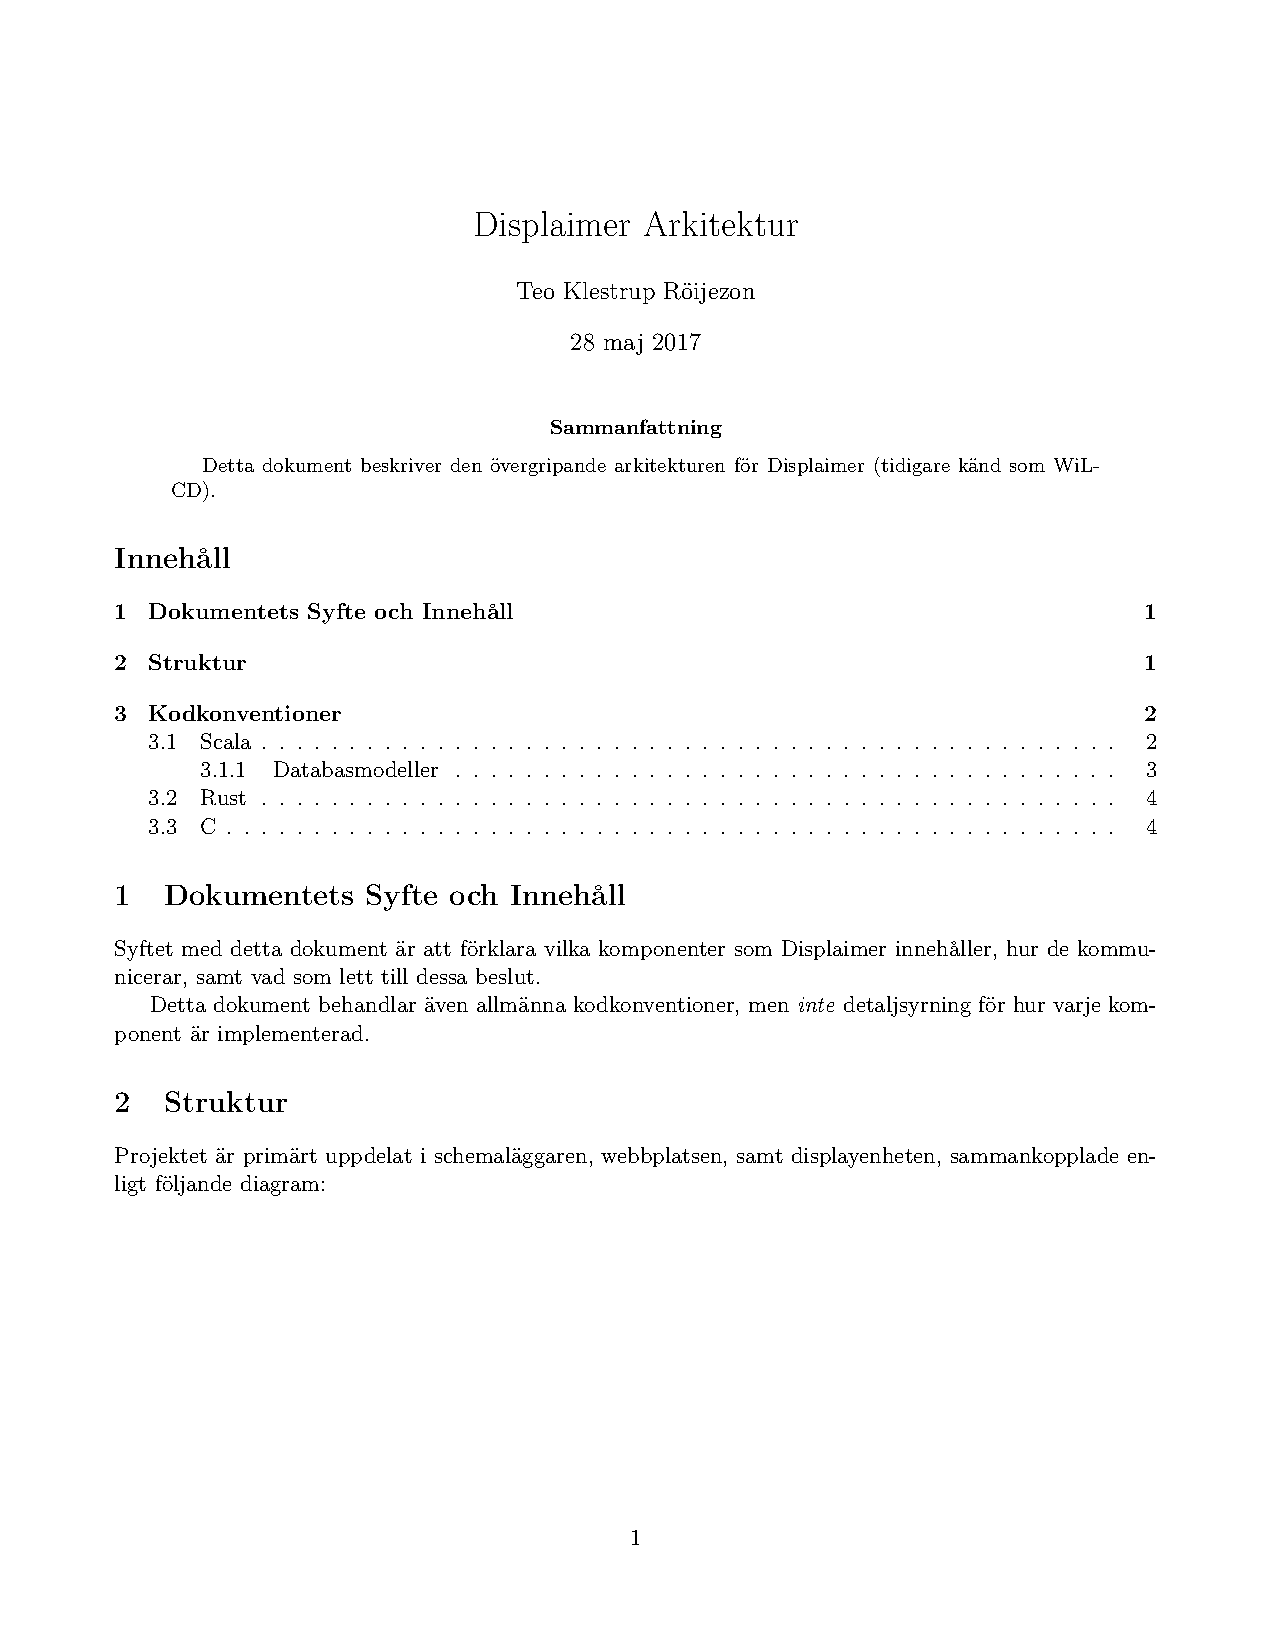
\includepdf[pages=-]{../../Arkitektur/Arkitektur}
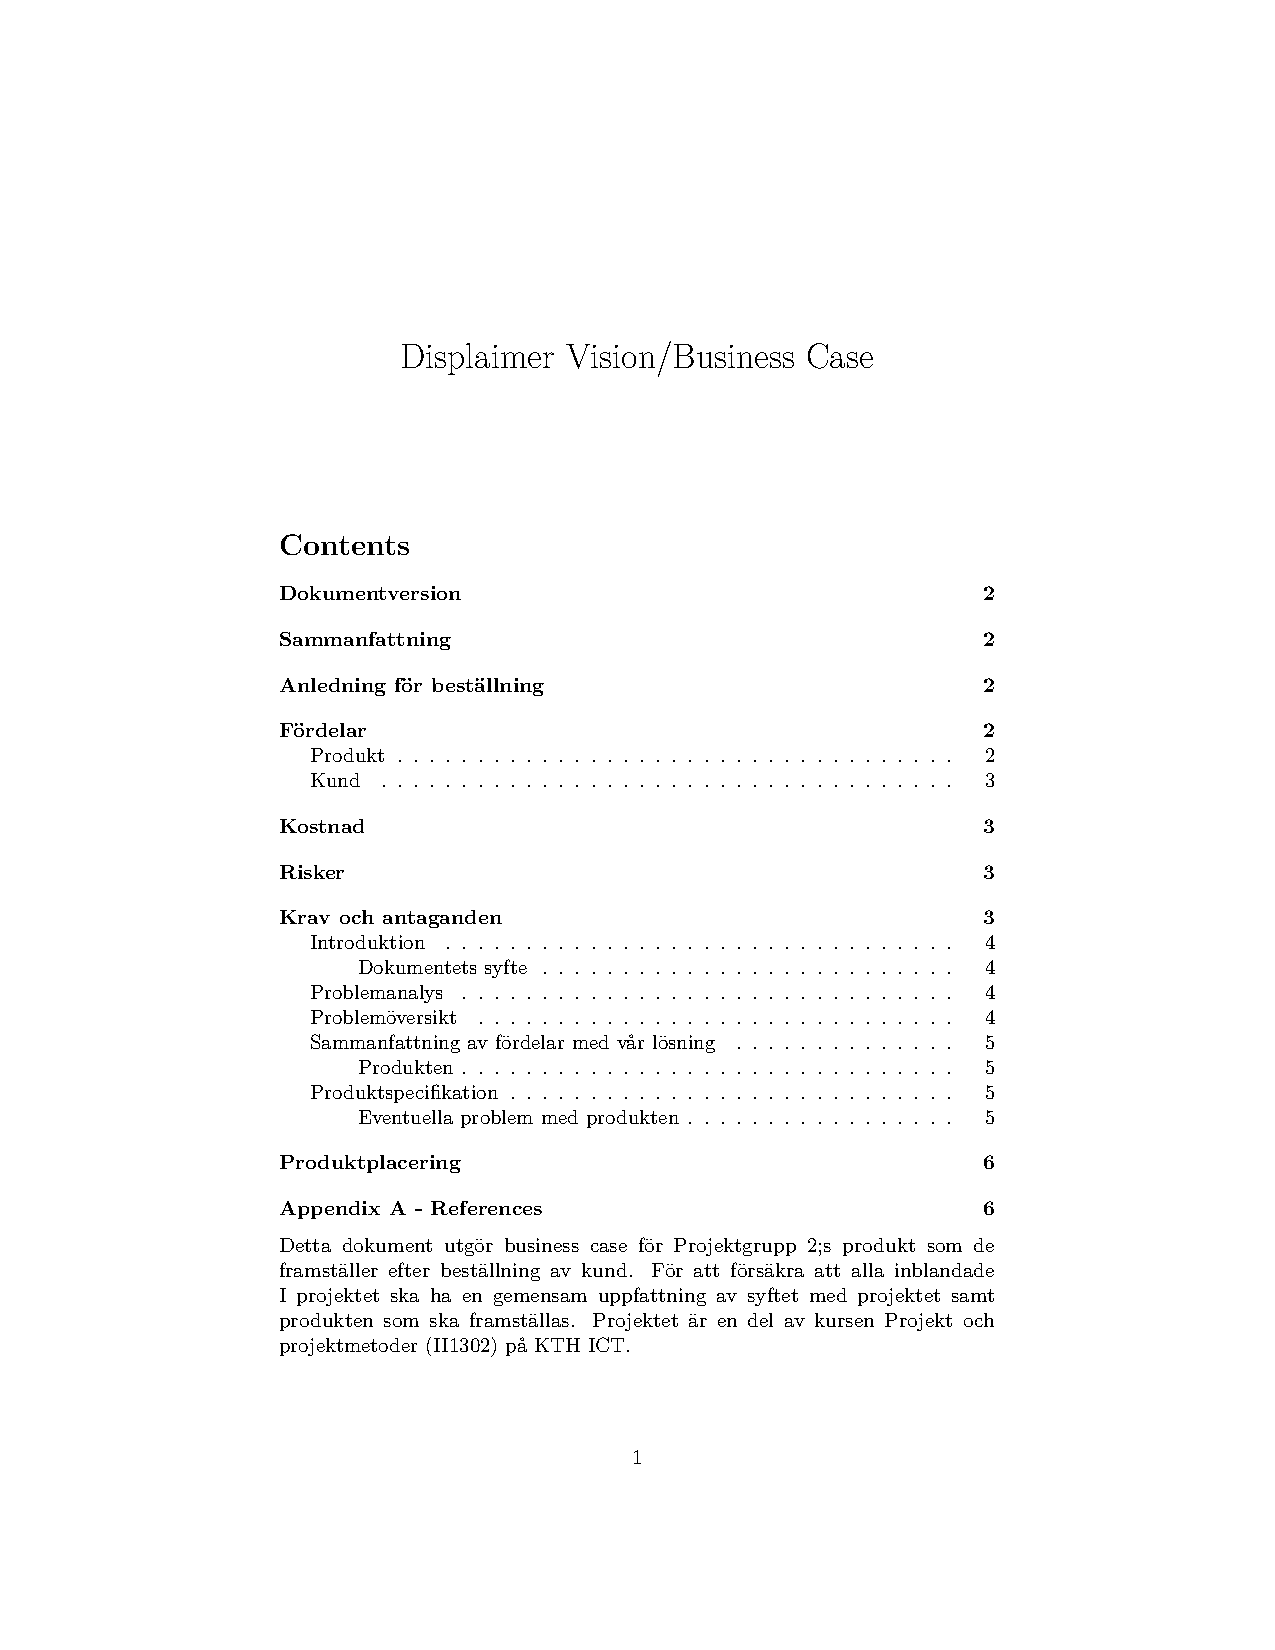
\includepdf[pages=-]{../Vision}
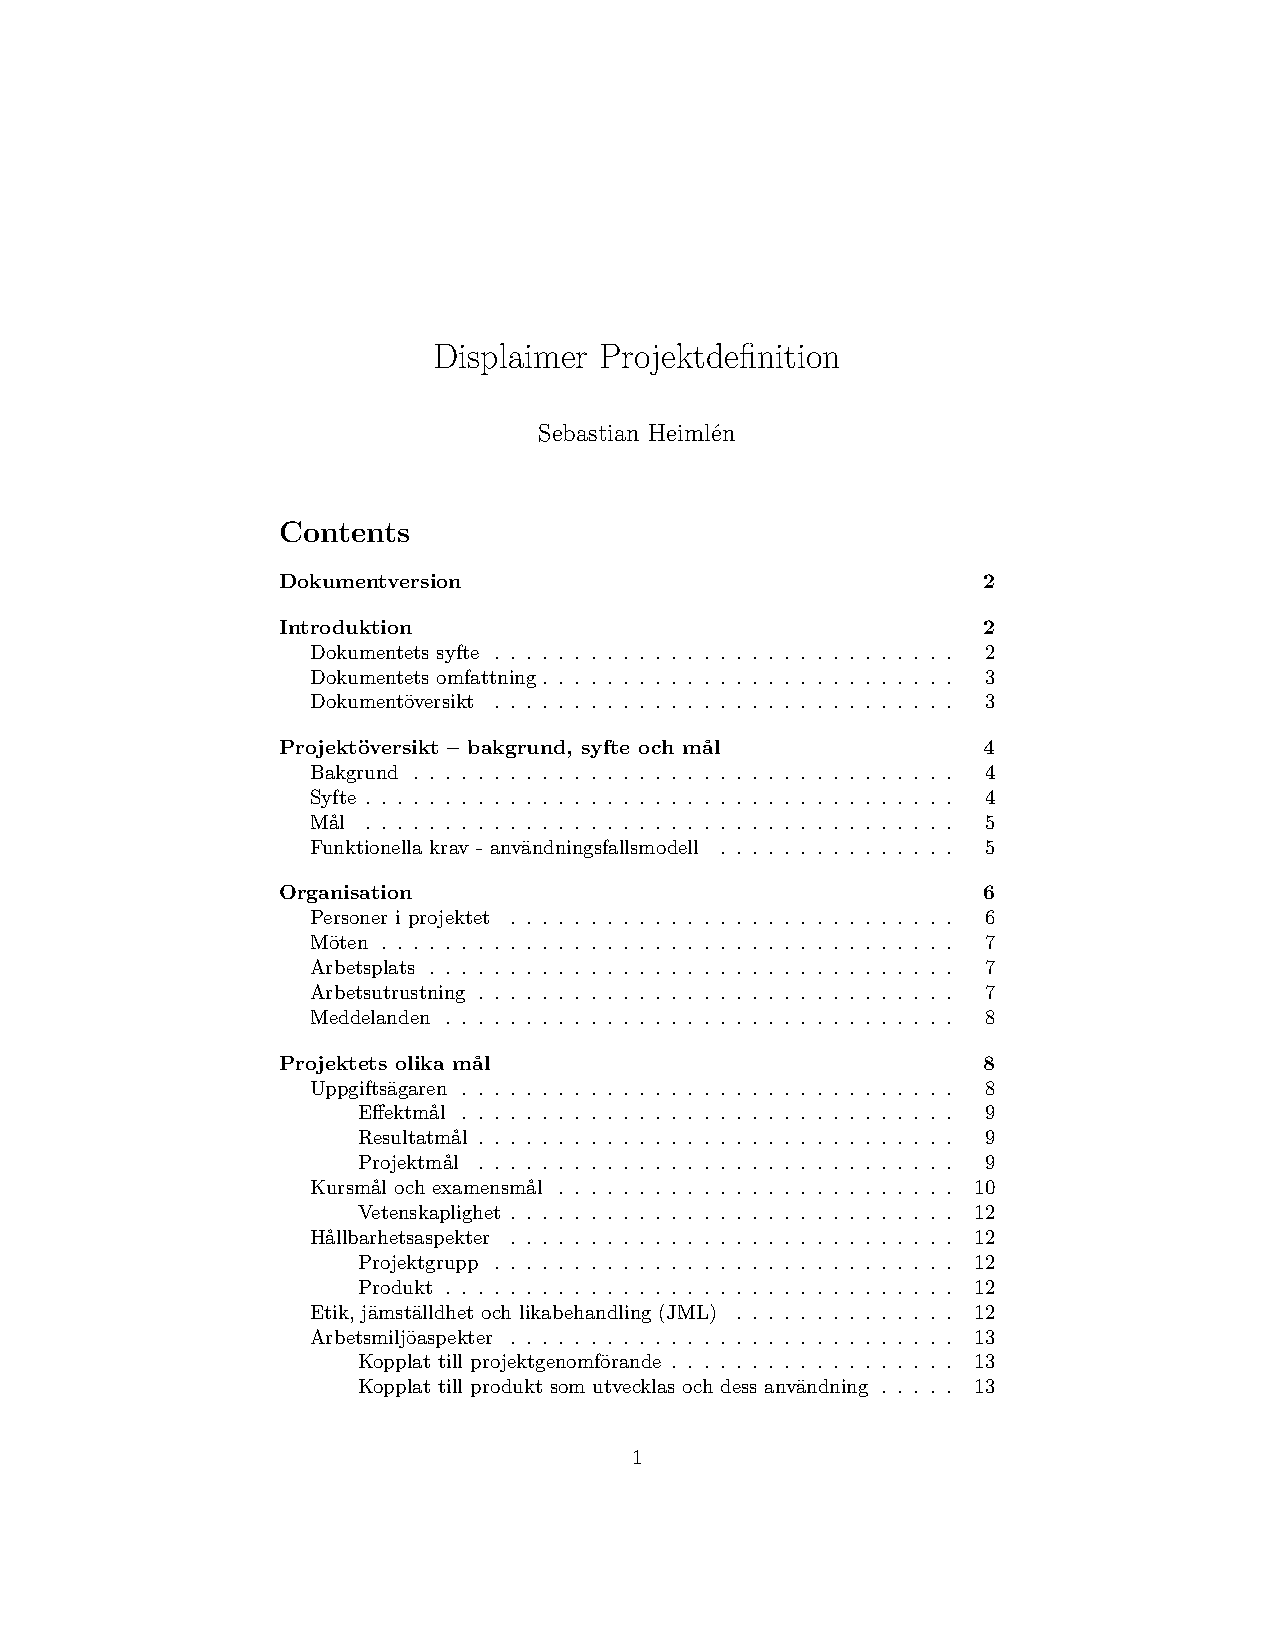
\includepdf[pages=-]{../Projektdefinition_Grupp2}

\section{Tekniska Specifikationer}
Se nästa sida.
% Bryt sidan ordentligt, annars överlappar sista sista sidan av den inkluderade pdfen
% med sista sidan av rapporten
\newpage
\null%
\newpage
% Kör pdfannotextractor (del av TeXLive) på varje inkluderad pdf så att
% länkar fortfarande fungerar
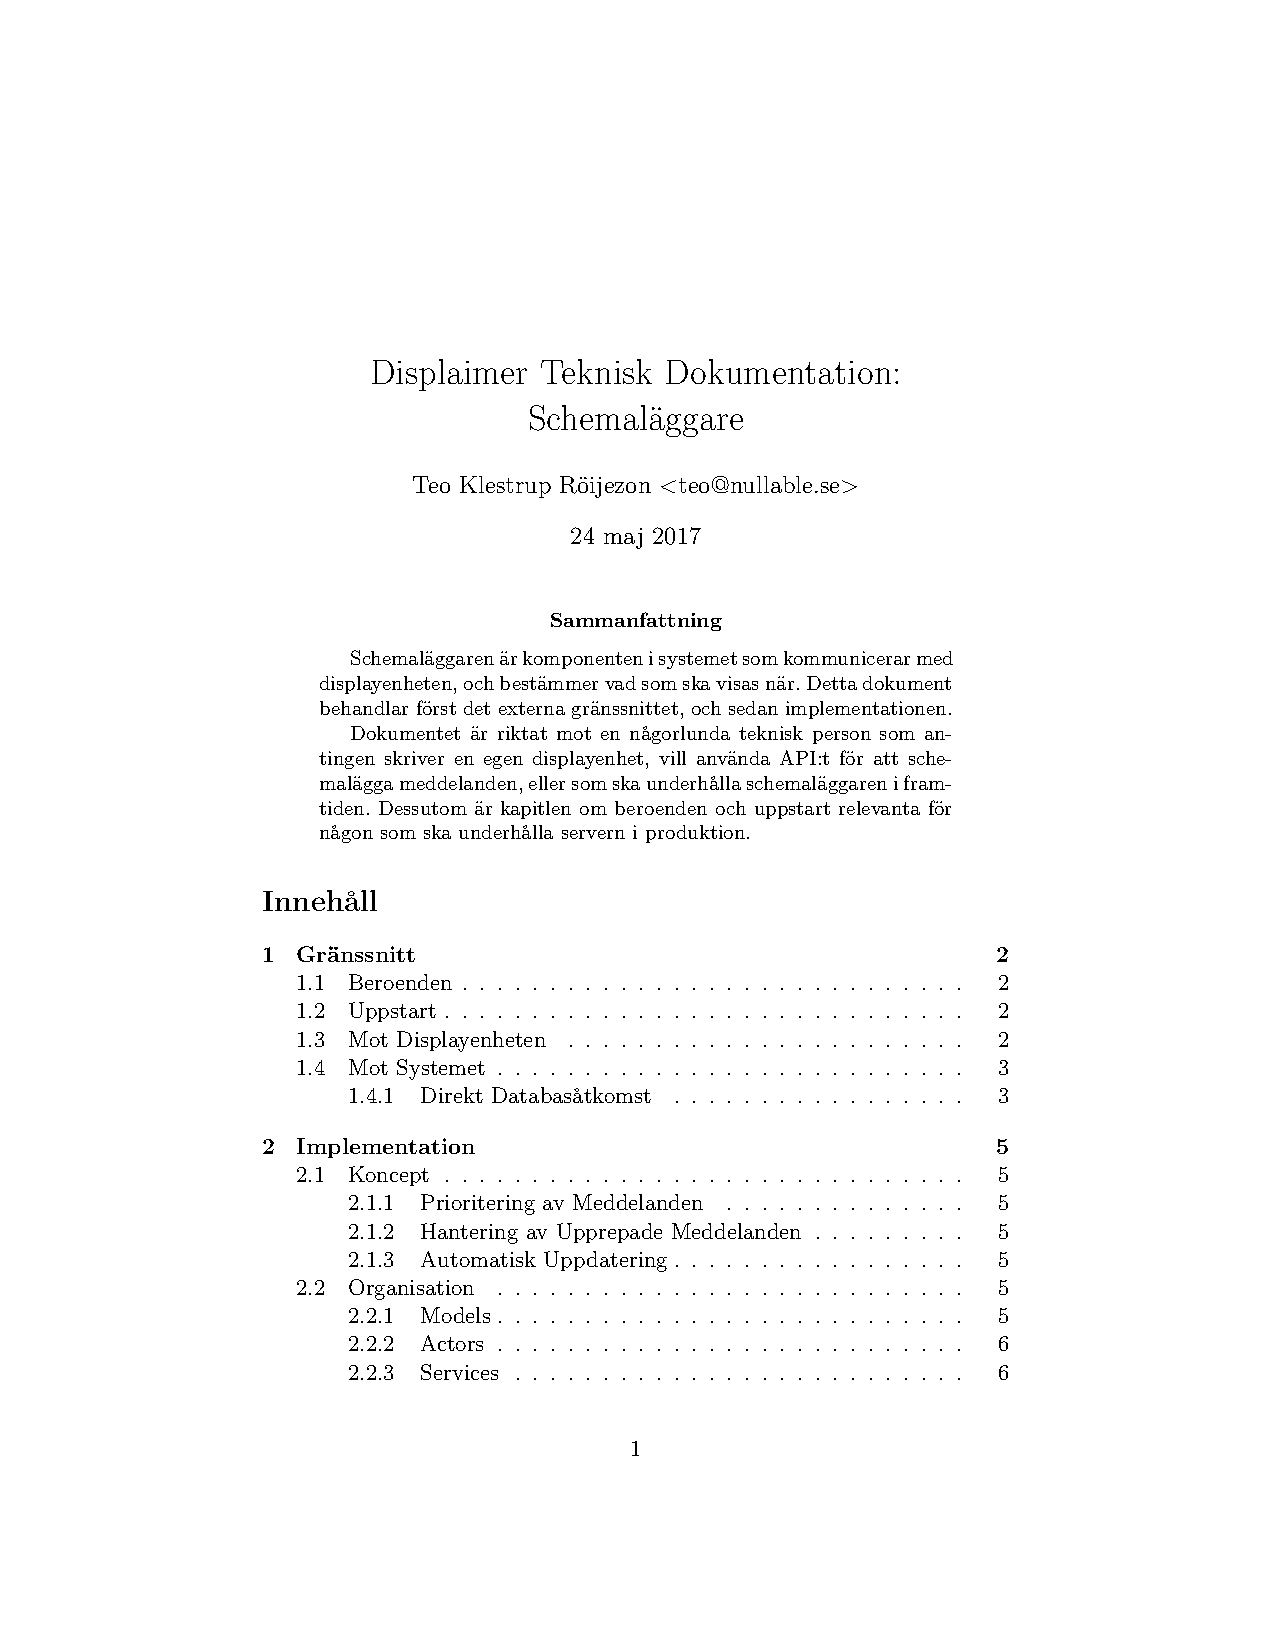
\includepdf[pages=-]{../Spec/Schemalaggare}
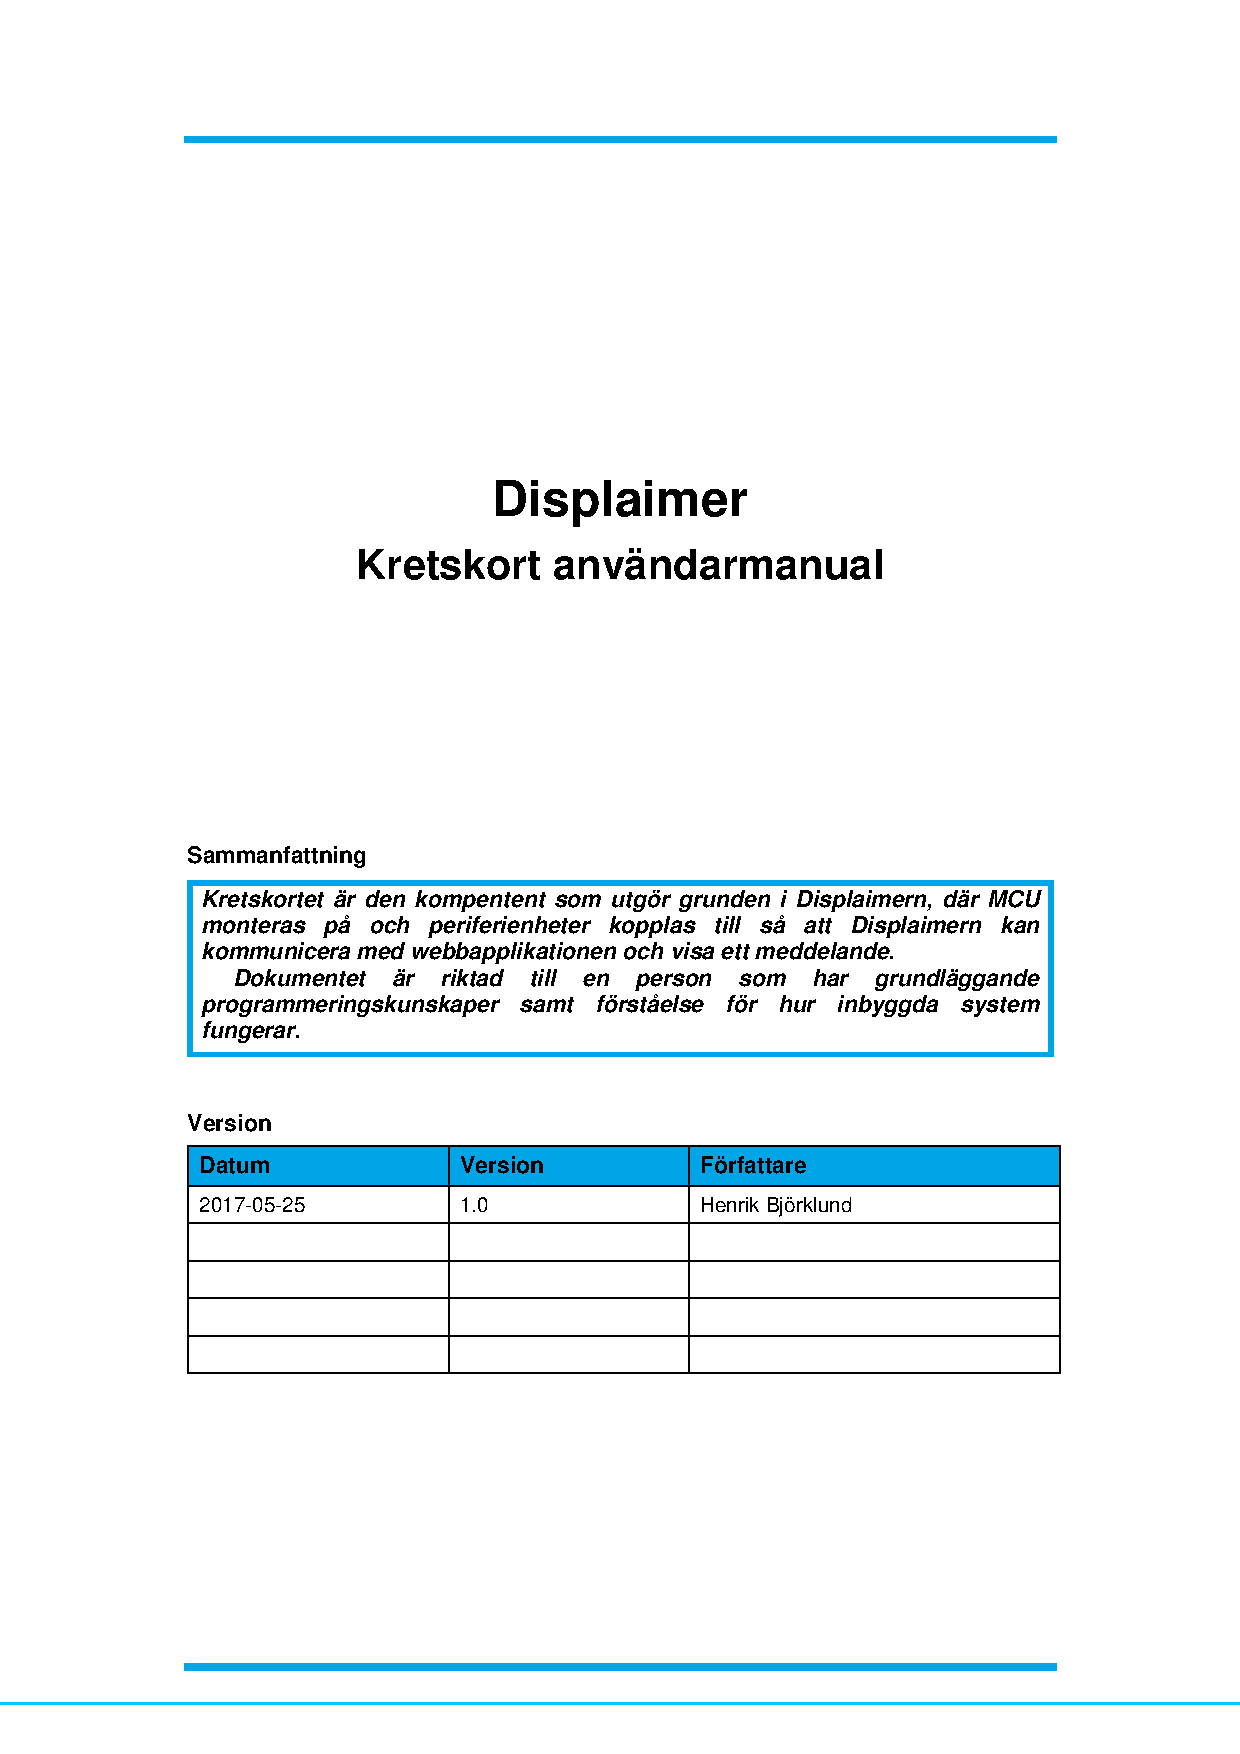
\includepdf[pages=-]{../Spec/TD_PCB}

% that's all folks
\end{document}
